\documentclass[dvipsnames, aspectratio=169]{beamer}
\usepackage[utf8]{inputenc}
\usepackage{listings}
\usepackage{comment}
\usepackage{soul}
%\usepackage{ulem}
\usepackage{subfig}
\usepackage{pgf-pie}
\setul{}{1pt}
\usepackage[oldenum, olditem]{paralist}
%allow even smaller text
\newcommand\tinytiny{\fontsize{4pt}{3}\selectfont}

\makeatletter
\let\old@lstKV@SwitchCases\lstKV@SwitchCases
\def\lstKV@SwitchCases#1#2#3{}
\makeatother
\usepackage{lstlinebgrd}
\makeatletter
\let\lstKV@SwitchCases\old@lstKV@SwitchCases

\lst@Key{numbers}{none}{%
    \def\lst@PlaceNumber{\lst@linebgrd}%
    \lstKV@SwitchCases{#1}%
    {none:\\%
     left:\def\lst@PlaceNumber{\llap{\normalfont
                \lst@numberstyle{\thelstnumber}\kern\lst@numbersep}\lst@linebgrd}\\%
     right:\def\lst@PlaceNumber{\rlap{\normalfont
                \kern\linewidth \kern\lst@numbersep
                \lst@numberstyle{\thelstnumber}}\lst@linebgrd}%
    }{\PackageError{Listings}{Numbers #1 unknown}\@ehc}}
\makeatother


%disclaimer for Sandia. uncomment and the whole blob goes away @ b80c116300122
\def\sandid{SAND2020-9315 TR}

% \title{Performance Portability with Kokkos}
\title{The Kokkos Lectures}

%BAD misuse of author field
\author{Module 8: Kokkos Kernels Math Library}


\usetheme{kokkos}

\newif\ifshort
\newif\ifmedium
\newif\iffull
\newif\ifnotoverview

\newcommand{\TutorialDirectory}{\texttt{Intro-Full}}
\newcommand{\ExerciseDirectory}[1]{\texttt{Exercises/#1/}}
\newcommand{\TutorialClone}{\texttt{Kokkos/kokkos-tutorials/\TutorialDirectory}}

\definecolor{darkgreen}{rgb}{0.0, 0.5, 0.0}
\definecolor{darkred}{rgb}{0.8, 0.0, 0.0}
\definecolor{orange}{rgb}{0.8, 0.33, 0.0}
\definecolor{purple}{rgb}{0.60, 0.20, 0.80}
\colorlet{bodyColor}{blue!20}
\colorlet{patternColor}{orange!30}
\colorlet{policyColor}{green!30}

% http://tex.stackexchange.com/questions/144448/color-a-text-line-in-a-code-lstlisting
\lstnewenvironment{code}[1][]%
{
  %with txfonts: OT1/txr/m/n/10
  %with default fonts: OT1/cmr/m/n/10
  %\fontfamily{cmr}\selectfont
  %\showthe\font
   \noindent
   \minipage{\linewidth}
   %\vspace{0.5\baselineskip}
   \lstset{mathescape, escapeinside={<@}{@>},
moredelim=**[is][{\btHL[fill=patternColor]}]{@pattern}{@pattern},
moredelim=**[is][{\btHL[fill=red!30]}]{@warning}{@warning},
moredelim=**[is][{\btHL[fill=policyColor]}]{@policy}{@policy},
moredelim=**[is][{\btHL[fill=bodyColor]}]{@body}{@body},
moredelim=**[is][{\btHL[fill=red!30]}]{@warning}{@warning},
moredelim=**[is][\color{black}]{@black}{@black},
moredelim=**[is][\color{blue}]{@blue}{@blue},
moredelim=**[is][\bf]{@bold}{@bold},
moredelim=**[is][\it]{@italic}{@italic},
moredelim=**[is][\color{boldblue}\bf]{@boldblue}{@boldblue},
moredelim=**[is][\color{red}]{@red}{@red},
moredelim=**[is][\color{green}]{@green}{@green},
moredelim=**[is][\color{gray}]{@gray}{@gray},
moredelim=**[is][\color{darkgreen}]{@darkgreen}{@darkgreen},
moredelim=**[is][\color{darkred}]{@darkred}{@darkred},
moredelim=**[is][\color{orange}]{@orange}{@orange},
moredelim=**[is][\color{purple}]{@purple}{@purple},
keywords={},
#1}
}
{
  \endminipage
  %\vspace{1.0\baselineskip}
}

\makeatletter
\newif\ifATOlinebackground
\lst@Key{linebackground}{\tiny}{\def\ATOlinebackground{#1}\global\ATOlinebackgroundtrue}
\makeatother

\lstnewenvironment{shell}[1][]{%
  \global\ATOlinebackgroundfalse
  \lstset{language=sh,%
    showstringspaces=false,
    aboveskip=0pt,
    frame=none,
    numbers=none,
    belowskip=2pt,
    breaklines=true,
    #1,
    }
  %\ifATOlinebackground
  \lstset{linebackgroundcolor={
    \ATOlinebackground
  }}
  %\fi
  }{}

\lstnewenvironment{cmake}[1][]{%
  \global\ATOlinebackgroundfalse
  \lstset{language=sh,%
    showstringspaces=false,
    aboveskip=0pt,
    frame=none,
    numbers=none,
    belowskip=2pt,
    breaklines=true,
    #1,
    }
  %\ifATOlinebackground
  \lstset{linebackgroundcolor={
    \ATOlinebackground
  }}
  %\fi
  }{}

\newcommand{\inlinecode}[1]{{\lstset{basicstyle=\ttfamily,keywordstyle={},showstringspaces=false}\lstinline$#1$}}
\newcommand{\inlineshell}[1]{{\lstset{basicstyle=\ttfamily,keywordstyle={},showstringspaces=false}\lstinline$#1$}}

\setbeamercolor{block title}{fg=white, bg=SandiaLightBlue}
\setbeamercolor{block body}{bg=lightgray}
\setbeamercolor{block title alerted}{fg=white, bg=SandiaRed}
\setbeamercolor{block body alerted}{bg=lightgray}



%\usepackage[texcoord,grid,gridunit=mm,gridcolor=red!10,subgridcolor=green!10]{eso-pic}
\usepackage[absolute,overlay]{textpos}





% http://tex.stackexchange.com/questions/8851/how-can-i-highlight-some-lines-from-source-code

\usepackage{pgf, pgffor}
\usepackage{listings}
\usepackage{lstlinebgrd} % see http://www.ctan.org/pkg/lstaddons

\makeatletter
%%%%%%%%%%%%%%%%%%%%%%%%%%%%%%%%%%%%%%%%%%%%%%%%%%%%%%%%%%%%%%%%%%%%%%%%%%%%%%
%
% \btIfInRange{number}{range list}{TRUE}{FALSE}
%
% Test in int number <number> is element of a (comma separated) list of ranges
% (such as: {1,3-5,7,10-12,14}) and processes <TRUE> or <FALSE> respectively

\newcount\bt@rangea
\newcount\bt@rangeb

\newcommand\btIfInRange[2]{%
    \global\let\bt@inrange\@secondoftwo%
    \edef\bt@rangelist{#2}%
    \foreach \range in \bt@rangelist {%
        \afterassignment\bt@getrangeb%
        \bt@rangea=0\range\relax%
        \pgfmathtruncatemacro\result{ ( #1 >= \bt@rangea) && (#1 <= \bt@rangeb) }%
        \ifnum\result=1\relax%
            \breakforeach%
            \global\let\bt@inrange\@firstoftwo%
        \fi%
    }%
    \bt@inrange%
}
\newcommand\bt@getrangeb{%
    \@ifnextchar\relax%
        {\bt@rangeb=\bt@rangea}%
        {\@getrangeb}%
}
\def\@getrangeb-#1\relax{%
    \ifx\relax#1\relax%
        \bt@rangeb=100000%   \maxdimen is too large for pgfmath
    \else%
        \bt@rangeb=#1\relax%
    \fi%
}

%%%%%%%%%%%%%%%%%%%%%%%%%%%%%%%%%%%%%%%%%%%%%%%%%%%%%%%%%%%%%%%%%%%%%%%%%%%%%%
%
% \btLstHL<overlay spec>{range list}
%
% TODO BUG: \btLstHL commands can not yet be accumulated if more than one overlay spec match.
%
\newcommand<>{\btLstHL}[2]{%
  \only#3{\btIfInRange{\value{lstnumber}}{#1}{\color{#2}\def\lst@linebgrdcmd{\color@block}}{\def\lst@linebgrdcmd####1####2####3{}}}%
}%
\makeatother






% http://tex.stackexchange.com/questions/15237/highlight-text-in-code-listing-while-also-keeping-syntax-highlighting
%\usepackage[T1]{fontenc}
%\usepackage{listings,xcolor,beramono}
\usepackage{tikz}

\makeatletter
\newenvironment{btHighlight}[1][]
{\begingroup\tikzset{bt@Highlight@par/.style={#1}}\begin{lrbox}{\@tempboxa}}
{\end{lrbox}\bt@HL@box[bt@Highlight@par]{\@tempboxa}\endgroup}

\newcommand\btHL[1][]{%
  \begin{btHighlight}[#1]\bgroup\aftergroup\bt@HL@endenv%
}
\def\bt@HL@endenv{%
  \end{btHighlight}%
  \egroup
}
\newcommand{\bt@HL@box}[2][]{%
  \tikz[#1]{%
    \pgfpathrectangle{\pgfpoint{1pt}{0pt}}{\pgfpoint{\wd #2}{\ht #2}}%
    \pgfusepath{use as bounding box}%
    \node[anchor=base west, fill=orange!30,outer sep=0pt,inner xsep=1pt, inner ysep=0pt, rounded corners=3pt, minimum height=\ht\strutbox+1pt,#1]{\raisebox{1pt}{\strut}\strut\usebox{#2}};
  }%
}
\makeatother



\usetikzlibrary{calc}
\usepackage{xparse}%  For \NewDocumentCommand

% tikzmark command, for shading over items
\newcommand{\tikzmark}[1]{\tikz[overlay,remember picture] \node (#1) {};}

\makeatletter
\NewDocumentCommand{\DrawBox}{s O{}}{%
    \tikz[overlay,remember picture]{
    \IfBooleanTF{#1}{%
        \coordinate (RightPoint) at ($(left |- right)+(\linewidth-\labelsep-\labelwidth,0.0)$);
    }{%
        \coordinate (RightPoint) at (right.east);
    }%
    \draw[red,#2]
      ($(left)+(-0.2em,0.9em)$) rectangle
      ($(RightPoint)+(0.2em,-0.3em)$);}
}

\NewDocumentCommand{\DrawBoxWide}{s O{}}{%
    \tikz[overlay,remember picture]{
    \IfBooleanTF{#1}{%
        \coordinate (RightPoint) at ($(left |- right)+(\linewidth-\labelsep-\labelwidth,0.0)$);
    }{%
        \coordinate (RightPoint) at (right.east);
    }%
    \draw[red,#2]
      ($(left)+(-\labelwidth,0.9em)$) rectangle
      ($(RightPoint)+(0.2em,-0.3em)$);}
}

\NewDocumentCommand{\DrawBoxWideBlack}{s O{}}{%
    \tikz[overlay,remember picture]{
    \IfBooleanTF{#1}{%
        \coordinate (RightPoint) at ($(left |- right)+(\linewidth-\labelsep-\labelwidth,0.0)$);
    }{%
        \coordinate (RightPoint) at (right.east);
    }%
    \draw[black,#2]
      ($(left)+(-\labelwidth,0.9em)$) rectangle
      ($(RightPoint)+(0.2em,-0.3em)$);}
}
\makeatother

\usetikzlibrary{positioning}

\usetikzlibrary{shapes}

\hypersetup{
    colorlinks=true,
    linkcolor=blue,
    filecolor=magenta,
    urlcolor=cyan,
}



\shortfalse
\mediumtrue
\fulltrue
\notoverviewtrue

\begin{document}

\begin{frame}
	\titlepage
\end{frame}

\begin{frame}[fragile]{Welcome to Kokkos}

\textbf{Online Resources}:

\begin{itemize}
        \item \url{https://github.com/kokkos}:
                \begin{itemize}
                        \item Primary Kokkos GitHub Organization
                \end{itemize}
        \item \url{https://github.com/kokkos/kokkos-tutorials/wiki/Kokkos-Lecture-Series}:
                \begin{itemize}
			\item{Slides, recording and Q\&A for the Lectures}
                \end{itemize}
        \item \url{https://kokkos.github.io/kokkos-core-wiki}:
                \begin{itemize}
                        \item Wiki including API reference
                \end{itemize}
        \item \url{https://kokkosteam.slack.com}:
                \begin{itemize}
                        \item Slack channel for Kokkos.
                        \item Please join: fastest way to get your questions answered.
                        \item Can whitelist domains, or invite individual people.
                \end{itemize}
\end{itemize}

\end{frame}


\begin{frame}[fragile]{Lecture Series Outline}

\begin{itemize}
        \item Module 1: Introduction, Building and Parallel Dispatch
        \item Module 2: Views and Spaces
        \item Module 3: Data Structures + MultiDimensional Loops
        \item Module 4: Hierarchical Parallelism
        \item Module 5: Tasking, Streams and SIMD
        \item Module 6: Internode: MPI and PGAS
        \item Module 7: Tools: Profiling, Tuning and Debugging
        \item \textbf{Module 8: Kernels: Sparse and Dense Linear Algebra}
        \item Module 9: Fortran inter-op
\end{itemize}

\end{frame}

\begin{frame}[fragile]{Module 7: Summary}

\textbf{Kokkos Tools:}
\begin{itemize}
  \item Kokkos Tools provide an instrumentation interface \textbf{KokkosP} and \textbf{Tools} to leverage it.
  \item The interface is \textbf{always available} - even in release builds.
  \item Zero overhead if no tool is loaded during the run.
  \item Dynamically load a tool via setting \texttt{KOKKOS\_TOOLS\_LIBS} environment variable.
  \item Set callbacks in code for tools compiled into the executable. 
\end{itemize}

\textbf{Kokkos Connector Tools:}
\begin{itemize}
  \item Connectors inject Kokkos specific information into vendor and academic tools.
  \item Helps readability of profiles.
  \item Removes need to put vendor specific instrumentation in codes.
  \item Growing list of tools support Kokkos natively.
\end{itemize}
\end{frame}

\begin{frame}[fragile]{Module 7: Summary}
\textbf{Kokkos Tuning Hooks enable more performance portability}
\begin{itemize}
  \item Avoid figuring out the right heuristic for every platform.
  \item Input variables descripte the problem scope.
  \item Output variables descripe the search space.
\end{itemize}

\textbf{Implementing your own tools is easy!}
\begin{itemize}
  \item Simply implement the needed C callback functions.
  \item Only implement what you need.
  \item The callback registration system allows to embed tools in applications.
\end{itemize}

\textbf{Static Analysis}
\begin{itemize}
  \item Have semantic checks going beyond C++ errors.
  \item Integrates into your editors.
\end{itemize}
\end{frame}

\begin{frame}[fragile]

  {\Huge Kokkos Kernels: Library Based Approach for Performance Portable Sparse/Dense linear algebra and Graph Kernels}

  \vspace{20pt}

  \textbf{Presented by:}

  Siva Rajamanickam, S. Acer, L. Berger-Vergiat, V. Dang, N. Ellingwood, E.
  Harvey, B. Kelley, K. Kim, C.R. Trott, J. Wilke

  \vspace{-20pt}

\end{frame}

%==========================================================================

\begin{frame}[fragile]{Module 8: Kernels Math Libraries}

\textbf{Kokkos Ecosystem for Performance Portability}

  \begin{columns}[t,onlytextwidth]
    \column{.75\textwidth}
    \begin{center}
      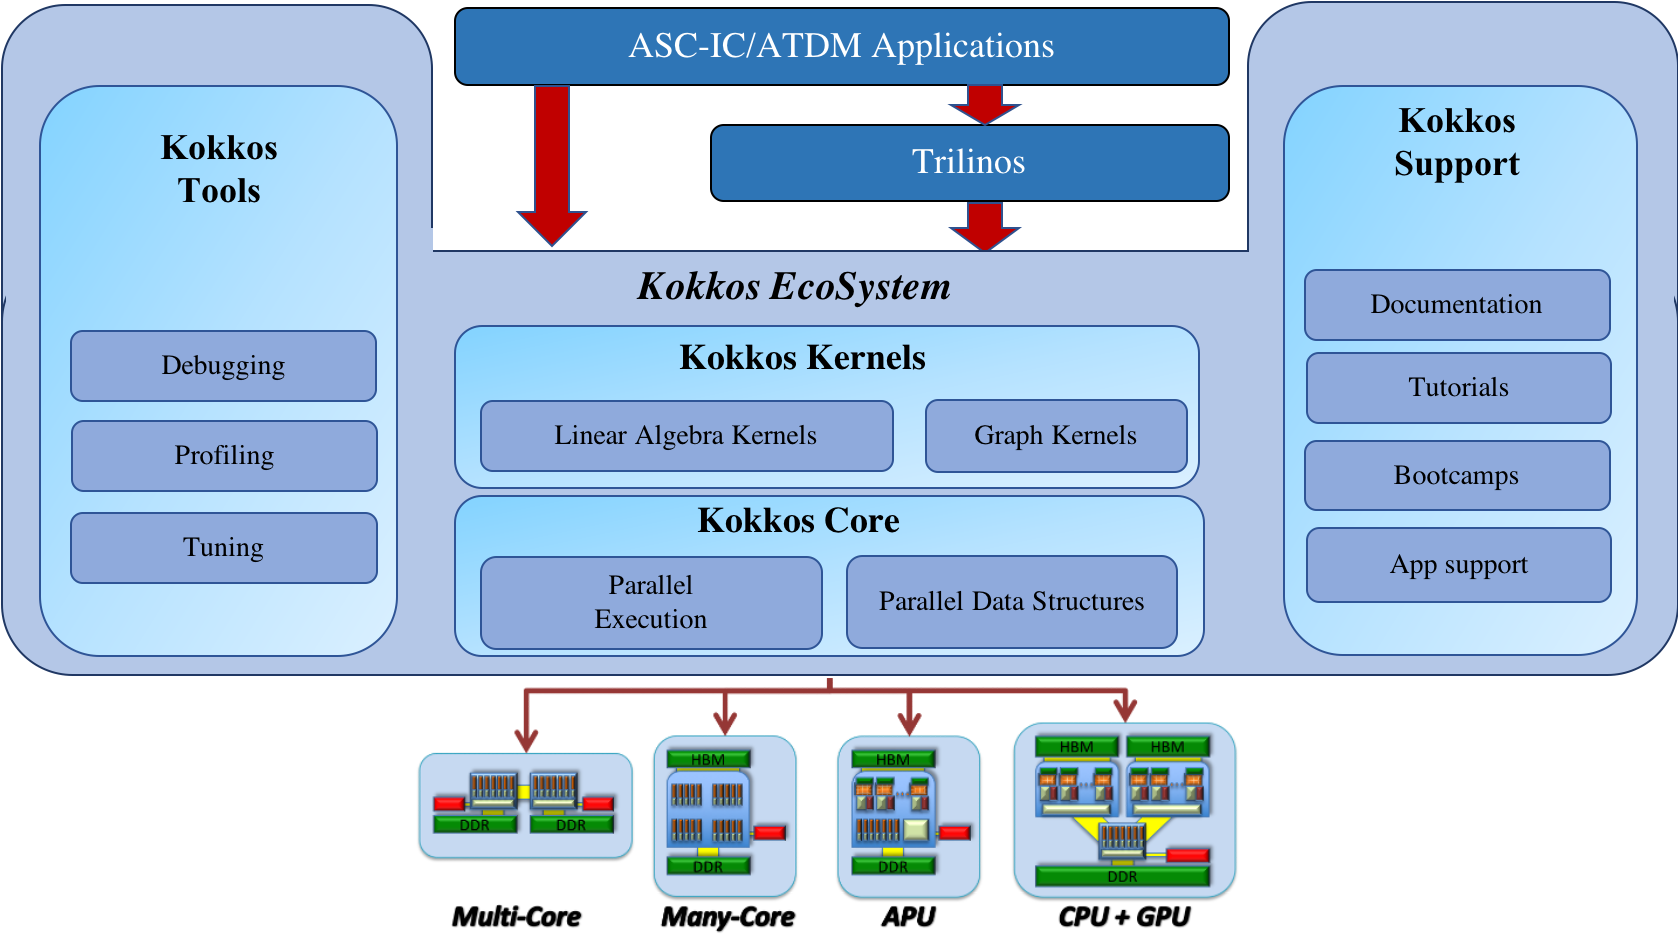
\includegraphics[width=0.95\textwidth]{figures/kernels-ecosystem}
    \end{center}

%    \begin{lstlisting}[frame=single, backgroundcolor=\color{blue!10}, basicstyle=\tiny, breaklines=true, boxpos=c]
%      Kokkos Ecosystem addresses complexity of supporting numerous many/multi-core architectures that are central to DOE HPC enterprise
%    \end{lstlisting}

    \column{.25\textwidth}
    \scriptsize{\textbf{Kokkos Core}: parallel patterns and data structures; supports several execution and memory spaces}
\\
    \scriptsize{\textbf{Kokkos Kernels}: performance portable BLAS; sparse, dense and graph algorithms}
\\
    \scriptsize{\textbf{Kokkos Tools}: debugging and profiling support}

%    \begin{lstlisting}[frame=single, backgroundcolor=\color{gray!10}, basicstyle=\tiny, breaklines=true]
%      Write - once using Kokkos for portable performance on different architectures
%    \end{lstlisting}

  \end{columns}

  \begin{lstlisting}[frame=single, backgroundcolor=\color{blue!10}, basicstyle=\tiny, breaklines=true, boxpos=c]
    Kokkos Ecosystem addresses complexity of supporting numerous many/multi-core architectures that are central to DOE HPC enterprise
  \end{lstlisting}

\end{frame}

%==========================================================================

\begin{frame}[fragile]{Focus of Kokkos Kernels}

Deliver \textbf{portable} sparse/dense linear algebra and graph kernels
\begin{itemize}
  \item These are the kernels that are in 80\% of time for most applications
  \item Key problems: Kernels might need different algorithms/implementations to get the best performance
  \item Ninja programming needs in addition to Kokkos
  \item Users of the kernels do not need to be ninja programmers
  \item \textbf{Focus on performance of the kernels on all the platforms of interest to DOE}
\end{itemize}

\begin{textblock*}{1.0\textwidth}(.1\textwidth,0.80\textheight)
  \begin{lstlisting}[frame=single, backgroundcolor=\color{blue!10}, basicstyle=\tiny, breaklines=true, boxpos=c]
    Kokkos Kernels delivers portable, high-performance kernels in a robust software ecosystem to support CSE applications
  \end{lstlisting}
\end{textblock*}

\end{frame}

\begin{frame}[fragile]{Focus of Kokkos Kernels}

Deliver \textbf{robust software ecosystem} for other software technology projects and applications
\begin{itemize}
  \item Production software capabilities that give high performance, portable and turn-key
  \item Tested on number of configurations nightly  (architectures, compilers, debug/optimized, programming model backend, complex/real, ordinal types...)
  \item Larger release/integration testing with Trilinos and applications
  \item Kokkos Support, github issues, tutorials, hackathons, user group meetings, slack
\end{itemize}

\begin{textblock*}{1.0\textwidth}(.1\textwidth,0.80\textheight)
  \begin{lstlisting}[frame=single, backgroundcolor=\color{blue!10}, basicstyle=\tiny, breaklines=true, boxpos=c]
    Kokkos Kernels delivers portable, high-performance kernels in a robust software ecosystem to support CSE applications
  \end{lstlisting}
\end{textblock*}

\end{frame}


\begin{frame}[fragile]{Focus of Kokkos Kernels}

Serve as \textbf{reference implementation} of key kernel needs of applications
\begin{itemize}
  \item Actively work with vendors to develop high performance implementation in their libraries
  \item Provide interface to vendor implementations where they are better
  \item Actively publish the algorithms so the community develops even better variations
\end{itemize}

\begin{textblock*}{1.0\textwidth}(.1\textwidth,0.80\textheight)
  \begin{lstlisting}[frame=single, backgroundcolor=\color{blue!10}, basicstyle=\tiny, breaklines=true, boxpos=c]
    Kokkos Kernels delivers portable, high-performance kernels in a robust software ecosystem to support CSE applications
  \end{lstlisting}
\end{textblock*}

\end{frame}

\begin{frame}[fragile]{Focus of Kokkos Kernels}

Actively partner with Applications to identify new opportunities for performance
\begin{itemize}
  \item Actively publish the algorithms so the community develops even better variations
  \item \textbf{Team-level dense, sparse linear algebra}
  \item \textbf{Team-level data structures (hashmap) and utilities (sorting) for better performance}
  \item \textbf{Fused Kernels}
  \item \textbf{Symbolic and Numeric separation in interface design}
\end{itemize}

\begin{textblock*}{1.0\textwidth}(.1\textwidth,0.80\textheight)
  \begin{lstlisting}[frame=single, backgroundcolor=\color{blue!10}, basicstyle=\tiny, breaklines=true, boxpos=c]
    Kokkos Kernels delivers portable, high-performance kernels in a robust software ecosystem to support CSE applications
  \end{lstlisting}
\end{textblock*}

\end{frame}


\begin{frame}[fragile]{Collaborations with Vendors}

\textbf{NVIDIA}
\begin{itemize}
  \item Summit on Summit meetings
  \item Biweekly work stream meetings to guide NVIDIA's math libraries plans
  \item Kernel requirements prioritized by application needs and milestones
  \item Long history of interaction as part of COE
  \item SpGEMM, GEMM, Solvers are all improved
\end{itemize}

\textbf{ARM}
\begin{itemize}
  \item Working with the math libraries team both on algorithms
  \item SpGEMM, SpMV, Batched linear algebra in ARM PL
\end{itemize}

%\begin{textblock*}{1.0\textwidth}(.1\textwidth,0.83\textheight)
%  \begin{lstlisting}[frame=single, backgroundcolor=\color{blue!10}, basicstyle=\tiny, breaklines=true, boxpos=c]
%    Kokkos Kernels team working with hardware vendors to support application 
%    needs on current and exascale platforms
%  \end{lstlisting}
%\end{textblock*}

\end{frame}

\begin{frame}[fragile]{Collaborations with Vendors}

\textbf{AMD}
\begin{itemize}
  \item Just started the interactions on sparse, dense, batched linear algebra kernels, and sparse solvers
  \item Kokkos backend under-development
  \item Kokkos Kernels will be the performance test case
\end{itemize}

\textbf{Intel}
\begin{itemize}
  \item Compact API on KNL
  \item Kokkos backend under development
  \item Kokkos Kernels will be the performance test case
\end{itemize}

\begin{textblock*}{1.0\textwidth}(.1\textwidth,0.83\textheight)
  \begin{lstlisting}[frame=single, backgroundcolor=\color{blue!10}, basicstyle=\tiny, breaklines=true, boxpos=c]
    Kokkos Kernels team working with hardware vendors to support application 
    needs on current and exascale platforms
  \end{lstlisting}
\end{textblock*}

\end{frame}


\begin{frame}[fragile]{Collaborations with ECP Applications}

\textbf{SPARC}:  state-of-the-art hypersonic unsteady hybrid structured/unstructured finite volume CFD code
\begin{itemize}
  \item \textbf{High performance line solvers; batched BLAS on CPUs and GPUs}
  \item \textbf{Performance-portable programming models}
\end{itemize}

\textbf{EMPIRE}: next-gen unstructured-mesh FEM PIC/multifluid plasma simulation code
\begin{itemize}
  \item Scalable solvers for electrostatic and electromagnetic systems for Trinity and Sierra architectures
  \item \textbf{Thread-scalable, performance-portable, on-node linear algebra kernels to support multigrid methods}
  \item \textbf{Performance-portable programming models}
  \item Non-linear solvers, discretization, and automatic differentiation approaches
\end{itemize}

%\begin{textblock*}{1.0\textwidth}(.1\textwidth,0.83\textheight)
%  \begin{lstlisting}[frame=single, backgroundcolor=\color{blue!10}, basicstyle=\tiny, breaklines=true, boxpos=c]
%    Kokkos Kernels integrated into several applications in an agile manner at 
%    all stages from requirements solicitation, designing kernels and integration
%  \end{lstlisting}
%\end{textblock*}

\end{frame}

\begin{frame}[fragile]{Collaborations with ECP Applications}

\textbf{Exawind}: next-gen wind simulation code
\begin{itemize}
  \item \textbf{Scalable solvers for Trinity and Sierra architectures}
  \item \textbf{Thread-scalable, performance-portable, on-node linear algebra kernels to support multigrid methods}
  \item \textbf{Performance-portable programming models}
\end{itemize}

\textbf{QMCPACK}: Electronic structure code with Quantum Monte Carlo Algorithms
\begin{itemize}
  \item Team level BLAS and LAPACK within the Kokkos ecssytem
\end{itemize}

\begin{textblock*}{1.0\textwidth}(.1\textwidth,0.83\textheight)
  \begin{lstlisting}[frame=single, backgroundcolor=\color{blue!10}, basicstyle=\tiny, breaklines=true, boxpos=c]
    Kokkos Kernels integrated into several applications in an agile manner at 
    all stages from requirements solicitation, designing kernels and integration
  \end{lstlisting}
\end{textblock*}

\end{frame}




\begin{frame}[fragile]{Module 8: Kernels Math Libraries (09/04)}

	\vspace{3pt}
	\textbf{Dense Linear Algebra (BLAS and Batched BLAS)}
	\begin{itemize}
        \item Motivation for BLAS/LAPACK functions
        \item Algorithm Specialization for Applications
        \item Calling BLAS/LAPACK functions
	\end{itemize}

	\vspace{3pt}
	\textbf{Sparse Linear Algebra}
	\begin{itemize}
        \item Sparse Containers (CrsMatrix, StaticCrsGraph, Vector)
        \item Sparse Matrix-Vector Multiplication (SpMV)
        \item Sparse Matrix-Matrix Addition (SpADD)
        \item Sparse Matrix-Matrix Multiplication (SpGEMM)
	\end{itemize}

  \vspace{3pt}
  \textbf{Graph Kernels}
  \begin{itemize}
        \item Distance-1 Graph Coloring
        \item Distance-2 Graph Coloring
        \item Bipartite Graph Partial Coloring
  \end{itemize}

\end{frame}

\begin{frame}[fragile]{Module 8: Kernels Math Libraries (09/04)}

	\vspace{3pt}
	\textbf{Sparse Solvers}
	\begin{itemize}
        \item Multicolor Gauss Seidel
        \item Cluster Gauss Seidel
        \item Two-Stage Gauss Seidel
        \item Sparse Incomplete LU Factorization (SpILUK)
        \item Sparse Triangular Solver (SpTRSV)
	\end{itemize}

	\vspace{3pt}
	\textbf{Build System}
	\begin{itemize}
        \item Using Kokkos Kernels in Your Project
        \item Configure, Build, and Install Kokkos Kernels
        \item Install with Spack
	\end{itemize}

\end{frame}


\begin{frame}[fragile]

  {\Huge BLAS and LAPACK}

  \vspace{20pt}

  \textbf{Learning objectives:}
  \begin{itemize}
    \item {Motivation for BLAS/LAPACK functions}
    \item {Algorithm Specialization for Applications}
    \item {Calling BLAS/LAPACK functions}
  \end{itemize}

  \vspace{-20pt}
\end{frame}

%==========================================================================
% Slide 2
\begin{frame}[fragile]{KokkosKernels BLAS/LAPACK Interface}

\vspace{-1em}
  \begin{columns}[t,onlytextwidth]
    \column{.50\textwidth}
      \begin{center}
        \textbf{KokkosKernels}
      \end{center}
    \column{.50\textwidth}
      \begin{center}
        \textbf{Vendor Libraries}
      \end{center}
  \end{columns}

%\noindent\makebox[\linewidth]{\rule{\paperwidth}{0.4pt}}
\noindent\rule{4in}{0.4pt}

  \begin{columns}[t,onlytextwidth]
    \column{.45\textwidth}
      \begin{flushleft}
      \vspace{-2em}
        \begin{itemize}
          \item \small{A single interface to vendor BLAS libraries on
          heterogenous computing platforms}
          \item \small{Support user-defined data type e.g., Automatic Differentiation,
          Ensemble, SIMD, types with Kokkos native implementation}
          \item \small{Customized performance solution for certain problem sizes}
          \item \small{Exploring new performance oriented interfaces}
        \end{itemize}
      \end{flushleft}
    \column{.10\textwidth}
    \column{.45\textwidth}
      \begin{flushright}
      \vspace{-2em}
        \begin{itemize}
          \item \small{A user needs to write a different function interface for
          different computing platforms e.g., MKL vs. CUBLAS}
          \item \small{Built-in real/complex data types and column/row major data
          layouts are only supported}
          \item \small{Code is highly optimized; in practice, higher performance is
          obtained from larger problem sizes}
        \end{itemize}
      \end{flushright}
  \end{columns}
\end{frame}

%==========================================================================
% Slide 3
\begin{frame}[fragile]{KokkosKernels BLAS/LAPACK Interface}
  \textbf{Algorithm Specialization for Applications}
  \begin{itemize}
    \item Dot-based GEMM
    \begin{itemize}
	    \item \small{GEMM is used for orthogonalizing Krylov multi-vectors (long skinny matrix)}
      \item \small{This particular problem shape does not perform well on CUBLAS}
      \item \small{Algorithm is specialized for this shape performing multiple dot
      products instead of running standard GEMM algorithms}
    \end{itemize}
    \item Compact Batched BLAS
    \begin{itemize}
      \item \small{Application wants to solve many instances of tiny square block dense
      matrices; e.g., block dimensions of 3, 5, 7, 9, 11, etc.}
      \item \small{Difficult to effectivley use wide vector length such as AVX512 for
      this small problem size}
      \item \small{A pack of block matrices are inter-leaved and solved simultaneously
      using vector instructions}
      \item \small{Code is trivially vectorized 100\% for the applied BLAS and LAPACK operations}
    \end{itemize}
  \end{itemize}
\end{frame}

%==========================================================================
% Slide 3
\begin{frame}[fragile]{KokkosKernels BLAS/LAPACK Interface}
  \textbf{Algorithm Specialization for Applications}
  \begin{itemize}
    \item Extended Blas 1 interface: see axpby, update (a, c, b, y, g, z)
    \begin{itemize}
      \item $y[i] = g*z[i] + b*y[i] + a*x[i]$
      \item Trilinos Tpetra interface used in Belos iterative solvers
    \end{itemize}
    \item See the wiki page for complete list of functions
    \begin{itemize}
      \item https://github.com/kokkos/kokkos-kernels/wiki
    \end{itemize}
  \end{itemize}
  \vspace{10pt}
  \begin{center}
    \framebox{\parbox[t][1.0cm]{9.0cm}{
      \centering
      \item KokkosKernels interacts with application teams and provides custom 
      performance solutions for their needs
    }}
  \end{center}
\end{frame}

%==========================================================================
% Begin NDE
% Slide 5
\begin{frame}[fragile]{KokkosKernels BLAS/LAPACK Interface}

\textbf {Recall the Kokkos Inner Product exercise:}

\begin{columns}[t,onlytextwidth]
  \column{.50\textwidth}
\begin{itemize}
%  \item Recall the Kokkos Inner Product exercise:
  \item Inner product $<y,A*x>$
  \begin{itemize}
    \item $y$ is $Nx1$, $A$ is $NxM$,\\ $x$ is $Mx1$
  \end{itemize}
  \item Early exercise code looked like

  \begin{code}[keywords={double,parallel_reduce,for,int}]
double result = 0;
Kokkos::parallel_reduce("yAz", N,
    KOKKOS_LAMBDA (int j, double &update) {
      double temp2 = 0;
      for (int i = 0; i < M; ++i) {
        temp2 += A(j, i) * x(i);
      }
      update += y(j) * temp2;
  }, result);
  \end{code}

\end{itemize}

  \column{.50\textwidth}
  \begin{flushright}
    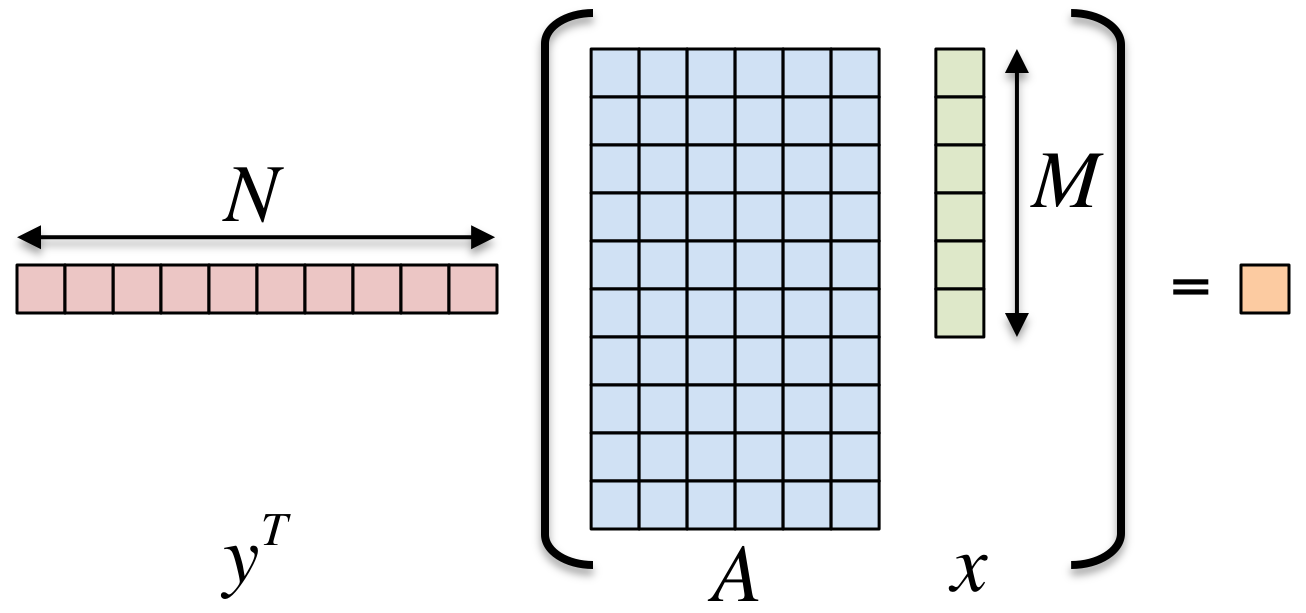
\includegraphics[width=0.85\textwidth]{figures/InnerProductExample_annotated}
  \end{flushright}
\end{columns}
\end{frame}

%Slide 6

\begin{frame}[fragile]{KokkosKernels BLAS/LAPACK Interface}

\textbf {This can be naturally expressed as two BLAS operations:} \\
In Matlab notation:
\vspace{-2em}

\begin{columns}[t,onlytextwidth]
  \column{.50\textwidth}
  \begin{center}
  \begin{code}[keywords={double,parallel_reduce,for,int}]
     // 1. gemv:
     Ytmp = A * x
  \end{code}
  \\
  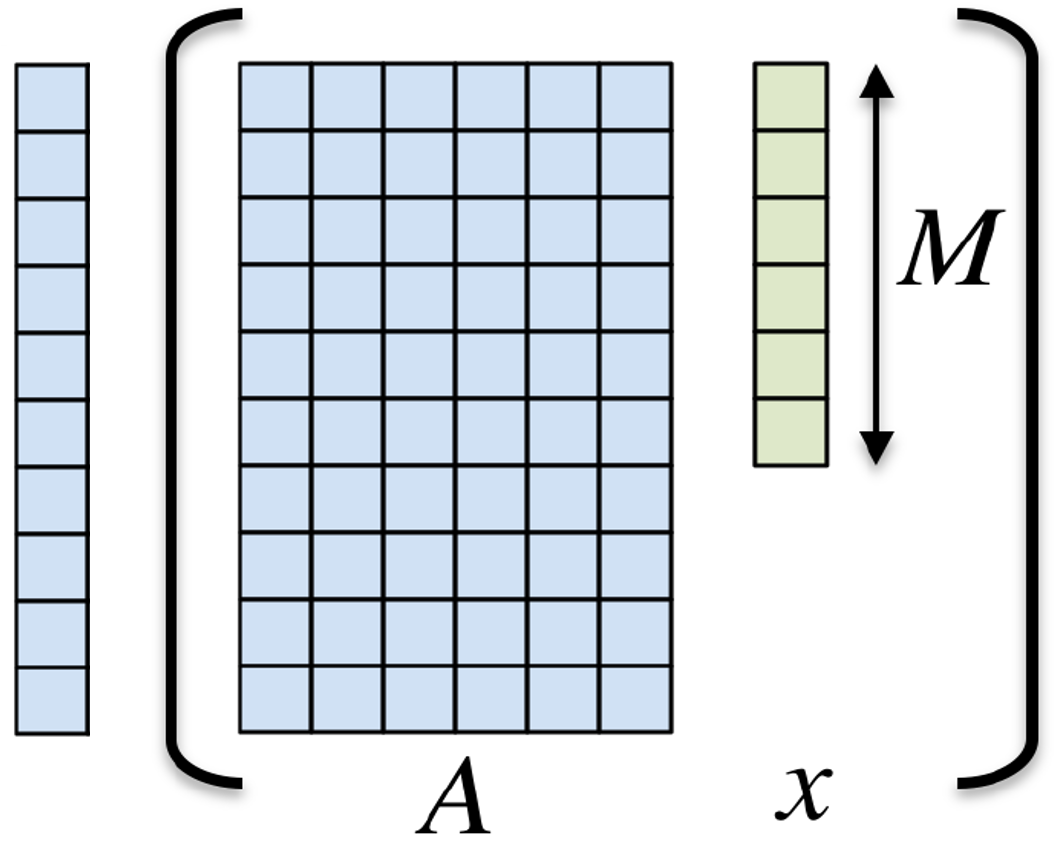
\includegraphics[width=0.5\textwidth]{figures/BLAS-A_times_x_res}
  \end{center}


  \column{.50\textwidth}
  \begin{center}
  \begin{code}[keywords={double,parallel_reduce,for,int}]
     // 2. dot:
     result = y'*Ytmp
  \end{code}
  \\
  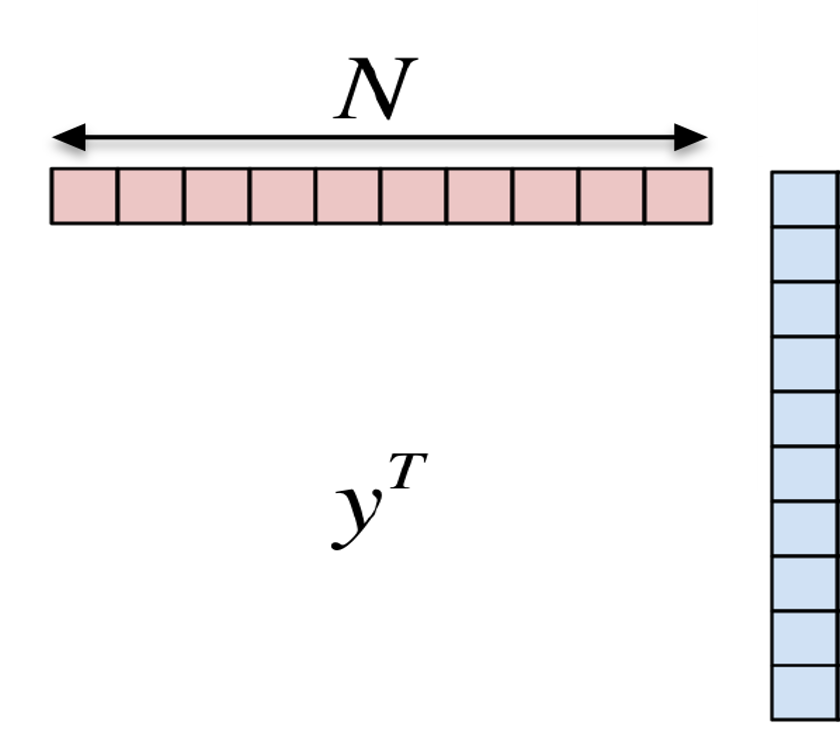
\includegraphics[width=0.5\textwidth]{figures/BLAS-y_dot_tmp}
  \end{center}
\end{columns}
\vspace{5pt}
\small{Different function signatures and APIs are used by different vendors}
\\
\small{  e.g., on Cuda: cublasDgemv and cublasDdot}
\end{frame}

% Slide 7

\begin{frame}[fragile]{KokkosKernels BLAS Interface: GEMV}

%\textbf {KokkosBLAS::gemv}

\begin{code}[basicstyle=\large, keywords={double,gemv,dot}]
KokkosBlas::gemv (mode, alpha, A, x, beta, y);
\end{code}

\textbf {Interface:}

\begin{itemize}
  \item mode [in] 
  \begin{itemize}
    \item "N" for non-transpose
    \item "T" for transpose
    \item "C" for conjugate transpose.
  \end{itemize}
  \item alpha [in] Input coefficient of A*x
  \item A [in] Input matrix, as a 2-D Kokkos::View
  \item x [in] Input vector, as a 1-D Kokkos::View
  \item beta [in] Input coefficient of y
  \item y [in/out] Output vector, as a nonconst 1-D Kokkos::View
\end{itemize}

\end{frame}

% Slide 8

\begin{frame}[fragile]{KokkosKernels BLAS Interface: DOT}

\begin{code}[basicstyle=\large, keywords={double,gemv,dot}]
result = KokkosBlas::dot(x,y);
\end{code}

\textbf {Single Interface:}

\begin{itemize}
  \item x [in] Input vector, as a 1-D Kokkos::View
  \item y [in] Input vector, as a 1-D Kokkos::View
  \item result [out] Scalar result on host
  \item This interface calls Kokkos::fence on all execution spaces
\end{itemize}

\begin{code}[basicstyle=\large, keywords={double,gemv,dot}]
KokkosBlas::dot(r,x,y);
\end{code}

\textbf {Single and Multi-vector Interface:}

\begin{itemize}
  \item x [in] Input (multi-)vector, as a 1-D or 2-D Kokkos::View
  \item y [in] Input (multi-)vector, as a 1-D or 2-D Kokkos::View
  \item r [in/out] Output result, as a rank-0 or 1-D Kokkos::View
  \item This interface is non-blocking.
\end{itemize}

\end{frame}


%==========================================================================
% Slide 9
\begin{frame}[fragile]{KokkosKernels BLAS/LAPACK Interface}

\vspace{-1em}

  \begin{columns}[t,onlytextwidth]
    \column{.50\textwidth}
      \begin{center}
        \textbf{KokkosKernels:}
      \end{center}
    \column{.50\textwidth}
      \begin{center}
        \textbf{User implementation:}
      \end{center}
  \end{columns}

%\noindent\makebox[\linewidth]{\rule{\paperwidth}{0.4pt}}
\noindent\rule{4in}{0.4pt}

  \begin{columns}[t,onlytextwidth]
    \column{.45\textwidth}
      \begin{flushleft}
      \vspace{-2em}
  \begin{code}[keywords={View,double,gemv,dot}, basicstyle=\tiny, breaklines=true]
Kokkos::View<double*> tmp("tmp", N);

KokkosBlas::gemv("N",alpha,A,x,beta,tmp);


double result = 0;

result = KokkosBlas::dot(y,tmp);
  \end{code}
      \end{flushleft}
    \column{.10\textwidth}
    \column{.45\textwidth}
      \begin{flushright}
      \vspace{-2em}
  \begin{code}[keywords={parallel_reduce,for,int,double}, basicstyle=\tiny, breaklines=true]
double result = 0;
Kokkos::parallel_reduce("yAx", N, 
 KOKKOS_LAMBDA (int j, double &update) { 
  double temp2 = 0;
   for (int i = 0; i < M; ++i) { 
     temp2 += A(j, i) * x(i);
   }
   update += y(j) * temp2;
 }, result);
  \end{code}
      \end{flushright}
  \end{columns}

\noindent\rule{4in}{0.4pt}

\vspace{-0.5em}
  \begin{columns}[t,onlytextwidth]
    \column{.45\textwidth}
      \begin{itemize}
        \vspace{-1em}
        \item{\scriptsize{Uses two BLAS functions}}
        \item{\scriptsize{Optionally interface to optimized vendor libraries}}
        \item{\scriptsize{For certain matrix shapes may choose specialized code path for performance}}
      \end{itemize}
    \column{.10\textwidth}
    \column{.45\textwidth}
      \begin{itemize}
        \vspace{-1em}
        \item{\scriptsize{Exploits a single level of parallelism only i.e., internal temp2 is summed sequentially}}
        \item{\scriptsize{Matrix-vector multiplication and dot product are fused in a single kernel}}
      \end{itemize}
  \end{columns}
\vspace{0.5em}
\scriptsize{Related exercise available at: \verb!Exercises/kokkoskernels/InnerProduct!}
%\item \tiny{\url{https://github.com/kokkos/kokkos-tutorials/tree/main/Exercises/kokkoskernels/InnerProduct/Begin}}

\end{frame}

\begin{frame}[fragile]{Summary}

  \textbf{Summary: BLAS/LAPACK}
  \begin{itemize}
  \item \small{Single interface for heterogeneous computing platforms}
  \item \small{Optimized vendor library interface when it is available}
  \item \small{Specialization of algorithms corresponding to application needs}
  \item \small{Native implementation supports strided data layout of a matrix}
  \end{itemize}
  
\end{frame}

%==========================================================================
% End NDE

\begin{frame}[fragile]

  {\Huge Batched BLAS and LAPACK}

  \vspace{20pt}

  \textbf{Learning objectives:}
  \begin{itemize}
    \item {Motivation for batched functions}
    \item {Two namespaces with BLAS and LAPACK functions}
    \item {Calling batched functions}
  \end{itemize}

  \vspace{-20pt}

\end{frame}

%==========================================================================
% Slide 11
\begin{frame}[fragile]{Parallel Batched BLAS/LAPACK Interface}

Batched BLAS/LAPACK is {\bf simple} i.e., BLAS/LAPACK in a parallel loop

  \begin{code}[frame=single, keywords={}, backgroundcolor=\color{brown!10}, basicstyle=\tiny]
auto A = Kokkos::View<double***>(''A'', N, Blk, Blk);
Kokkos::parallel_for( RangePolicy(N), /// users' parallel execution policy
  KOKKOS_LAMBDA(int &i) {
  auto AA = Kokkos::subview(A, i, ALL, ALL);
  KokkosBatched::SerialLU(AA);  /// functor-level interface
});
  \end{code}
\vspace{1pt}
Kokkos batched BLAS/LAPACK is made up of following two components
\begin{itemize}
\item Kokkos parallel execution policy with \verb|parallel_for|
\item A functor-level interface to be used in \verb|operator()|
\end{itemize}
\vspace{1pt}
Hierarchical functor interface is required matching to Kokkos' hierarchical parallelism

\end{frame}
  
\begin{frame}[fragile]{Layered Hierarchical Functor-level Interface}

  {\bf Serial Interface}
  \begin{itemize}
  \item \small{can be used in a flat \verb|parallel_for| i.e., \verb|Kokkos::RangePolicy|}
  \item \small{can be used in the most inner loop of nested \verb|parallel_for|'s}
  \end{itemize}
  \begin{columns}[t,onlytextwidth]
    \column{.475\textwidth}
  \textbf{\tiny{Serial with RangePolicy}}
  \begin{code}[frame=single, keywords={}, backgroundcolor=\color{brown!10}, basicstyle=\tiny, breaklines=true]
parallel_for(RangePolicy, 
 KOKKOS_LAMBDA(int &idx){
   KokkosBatched::SerialDoThing();
}); 
  \end{code}

    \column{.05\textwidth}
    \column{.475\textwidth}
  \textbf{\tiny{Serial in Hierarchical parallel loops}}
  \begin{code}[frame=single, keywords={}, backgroundcolor=\color{brown!10}, basicstyle=\tiny, breaklines=true]
parallel_for(TeamPolicy,
 KOKKOS_LAMBDA(member_type &member){
   parallel_for(TeamThreadRange) {
     parallel_for(ThreadVectorRange) {
       KokkosBatched::SerialDoSomething();
}); }); }); 
  \end{code}
  \end{columns}
\end{frame}

\begin{frame}[fragile]{Layered Hierarchical Functor-level Interface}

  {\bf TeamVector Interface}
  \begin{itemize}
  \item \small{internally uses two nested \verb|parallel_for| with \verb|TeamThreadRange| and \verb|ThreadVectorRange|}
  \item \small{requires the member (thread communicator) as an input argument}
  \end{itemize}
  \textbf{\tiny{TeamVector with TeamPolicy}}
  \begin{code}[frame=single, keywords={}, backgroundcolor=\color{brown!10}, basicstyle=\tiny, breaklines=true]
parallel_for(TeamPolicy, 
 KOKKOS_LAMBDA(member_type &member){
   KokkosBatched::TeamVectorDoSomething(member);
}); 
  \end{code}
\end{frame}

\begin{frame}[fragile]{Layered Hierarchical Functor-level Interface}

  {\bf Team Interface}
  \begin{itemize}
  \item \small{internally use \verb|TeamThreadRange| only}
  \item \small{in general is used with SIMD or Ensemble types where vector parallelism is expressed within the type}
  \item \small{can include \verb|ThreadVectorRange|}
  \end{itemize}
  \begin{columns}[t,onlytextwidth]
    \column{.475\textwidth}
  \textbf{\tiny{Team without ThreadVectorRange}}
  \begin{code}[frame=single, keywords={}, backgroundcolor=\color{brown!10}, basicstyle=\tiny, breaklines=true]
parallel_for(TeamPolicy, 
  KOKKOS_LAMBDA(member_type &member){
  KokkosBatched::TeamDoThing(member);
}); 
  \end{code}

    \column{.05\textwidth}
    \column{.475\textwidth}
  \textbf{\tiny{Team with ThreadVectorRange outside}}
  \begin{code}[frame=single, keywords={}, backgroundcolor=\color{brown!10}, basicstyle=\tiny, breaklines=true]
parallel_for(TeamPolicy,
 KOKKOS_LAMBDA(member_type &member){
   parallel_for(ThreadVectorRange) {
     KokkosBatched::TeamDoSomething(member);
}); }); 
  \end{code}
  \end{columns}
\end{frame}

%==========================================================================
\begin{frame}[fragile]{User Composable Batched BLAS and LAPACK}

  \textbf{} \\
  \vspace{26pt}
  Consider a batched \textbf{block matrix inversion} which can be used for a block
  Jacobi solver. \\
\end{frame}

%==========================================================================
\begin{frame}[fragile]{User Composable Batched BLAS and LAPACK}

  \textbf{KokkosKernels} \\
  \vspace{10pt}
  %\begin{tabular}{|p{3.6cm}|p{3.6cm}|}
  %  KokkosKernels  &  Vendor Libraries \\
    \begin{code}[keywords={parallel_for,auto,const,double}]
      using ViewTypeAs = Kokkos::View<double***>;


      using ScratchSpaceView = Kokkos::View<double*,
        Kokkos::DefaultExecutionSpace::scratch_memory_space,
        Kokkos::MemoryTraits<Kokkos::Unmanaged>>;
    \end{code}
  \end{frame}
  \begin{frame}[fragile]{User Composable Batched BLAS and LAPACK}

  \textbf{KokkosKernels} \\
    \begin{code}[keywords={parallel_for,auto,const,double}]
      ViewTypeAs As("As", N, Blk, Blk);
      Kokkos::parallel_for(TeamPolicy,
        KOKKOS_LAMBDA(member_type &member) {
          auto A = Kokkos::subview(As, i, ALL, ALL);
          auto T = ScratchSpaceView(member, Blk, Blk);
          KokkosBatched::TeamVectorLU(member, A);
          KokkosBatched::TeamVectorCopy(member, T, A);
          KokkosBatched::TeamVectorSetIdentity(member, A);
          KokkosBatched::TeamVectorLowerTrsm(member, T, A);
          KokkosBatched::TeamVectorUpperTrsm(member, T, A);
      });
    \end{code}
    \begin{itemize}
      \item \small{Multiple BLAS/LAPACK operations can be fused in a single kernel}
      \item \small{Temporal locality via single kernel launch}
      \item \small{Local cache memory can be used as scratch space}
      \item \small{Team size can be tuned for problem}
      \item \small{Poor performance when poorly tuned}
    \end{itemize}
\end{frame}

%==========================================================================
\begin{frame}[fragile]{User Composable Batched BLAS and LAPACK}

  \textbf{Vendor Libraries} \\
  \vspace{10pt}
  %\begin{tabular}{|p{3.6cm}|p{3.6cm}|}
  %  KokkosKernels  &  Vendor Libraries \\
    \begin{code}[keywords={}]
      As = Kokkos::View<double***>("As", N, Blk, Blk);
      Ts = Kokkos::View<double***>("Ts", N, Blk, Blk);
      batch_parallel_lu(As);
      batch_parallel_copy(Ts, As);
      batch_parallel_set_identity(As);
      batch_parallel_lower_trsm(Ts, As);
      batch_parallel_upper_trsm(Ts, As);
      
      /// or if you are lucky to find an inversion routine,
      batch_parallel_invert(As, Ts);
    \end{code}
    \begin{itemize}
      \item \small{Each batched kernel is highly optimized}
      \item \small{In a sequence of batch operations, the workflow can be suboptimal}
      \item \small{Multiple kernel launches can cause increased latency cost and more memory traffic}
    \end{itemize}
\end{frame}

%==========================================================================
\begin{frame}[fragile]{Two namespaces with BLAS and LAPACK functions}
  \textbf{KokkosBlas namespace} \\
  \vspace{10pt}
  \begin{itemize}
    \item \textbf{KokkosBlas:} device-level functions with optional TPL support
    \begin{itemize}
      \item \textit{Intended Use Case:}
      \begin{itemize}
        \item Caller uses the entire device execution space for solving a single dense problem
        \item For performance, the problem should be large enough to exploit the entire device
      \end{itemize}
      \item \textit{Blocking behavior:}
      \begin{itemize}
        \item On GPUs, non-blocking by default with some exceptions of norms
        where the result is requested from host
      \end{itemize}
    \end{itemize}
  \end{itemize}
\end{frame}

%==========================================================================
\begin{frame}[fragile]{Two namespaces with BLAS and LAPACK functions}
  \textbf{KokkosBatched namespace} \\
  \vspace{10pt}
  \begin{itemize}
    \item \textbf{KokkosBatched:} functor level functions
    \begin{itemize}
      \item \textit{Intended Use Case:}
      \begin{itemize}
        \item Caller is within parallel kernel body with a batch of input vectors
      \end{itemize}
      \item \textit{Multiple Interfaces: Serial, Team, TeamVector}
      \begin{itemize}
        \item Serial: no nested parallelism is used internally
        \item Team: one-level nested parallelism is used with \textit{TeamThreadRange}

        %%\begin{code} Kokkos::TeamThreadRange \end{code}
        \item TeamVector: two-level nested parallelism is used with \textit{TeamThreadRange and TeamVectorRange}

        %\begin{code} Kokkos::TeamThreadRange and Kokkos::TeamVectorRange \end{code}
      \end{itemize}
    \end{itemize}
  \end{itemize}
\end{frame}

%==========================================================================
\begin{frame}[fragile]{KokkosBatched interfaces - TeamGemm}
  \Huge {Exercise: TeamGemm}
\end{frame}

%==========================================================================
\begin{frame}[fragile]{KokkosBatched interfaces - TeamGemm}
  \begin{itemize}
    \item Recall Kokkos nested parallelism
    \item Exercise: $C = \beta * C + \alpha * A * B$
    \begin{itemize}
      \item $C$ is $P x M x N$
      \item $A$ is $P x M x K$
      \item $B$ is $P x K x N$
      \item $\beta$ and $\alpha$ are scalars
    \end{itemize}
  \end{itemize}
  \vspace{10pt}
  \begin{center}
    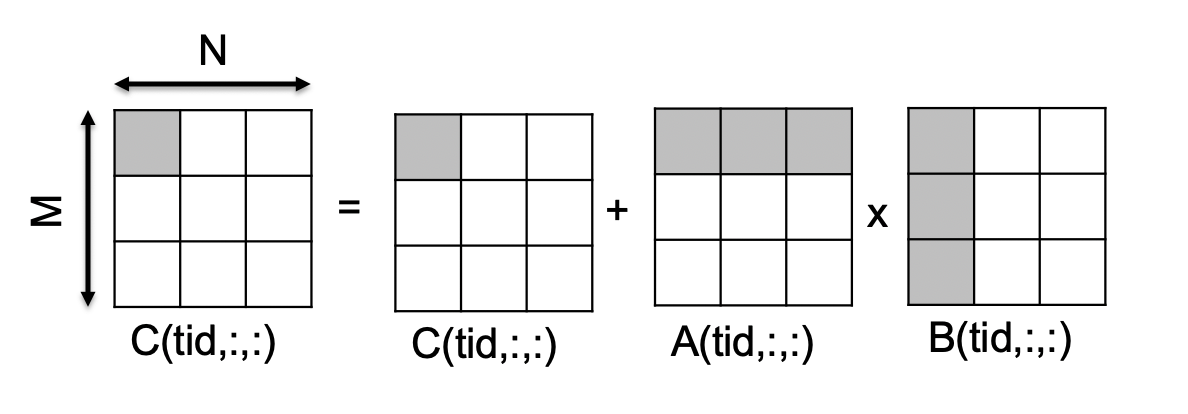
\includegraphics[width=0.65\textwidth]{figures/TeamGemm}
  \end{center}
\end{frame}

%==========================================================================
\begin{frame}[fragile]{KokkosBatched interfaces - TeamGemm}
  \begin{code}[keywords={parallel_for,auto,const,int}]
    Kokkos::parallel_for("teamGemmOuter", 
      Kokkos::TeamPolicy<ExecutionSpace>(nTeam, teamSize),
      KOKKOS_LAMBDA (const member_type &member) {
        const int tid = member.league_rank();
        // Each team performs a single TeamGemm
        Kokkos::parallel_for("teamGemmInner",
          Kokkos::TeamThreadRange(member, thisTeamsRangeSize),
          [=] (const unsigned int ij) {
            const int i = ij/N, j = ij%N;
            // each thread computes C(tid,i,j)
        });
    });
  \end{code}
  \vspace{10pt}
  \begin{center}
    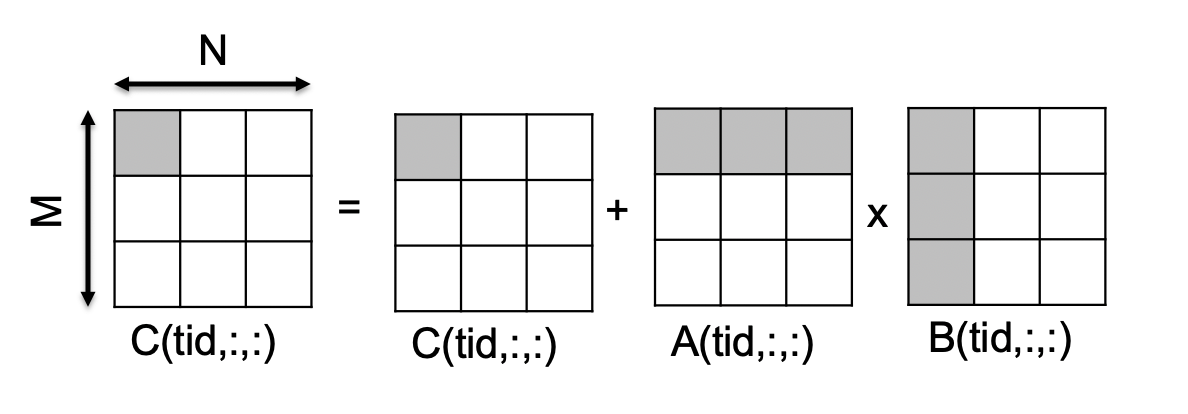
\includegraphics[width=0.65\textwidth]{figures/TeamGemm}
  \end{center}
\end{frame}

%==========================================================================
\begin{frame}[fragile]{KokkosBatched interfaces - TeamGemm}
  \textbf{This can be naturally expressed using the TeamGemm interface} \\
  \begin{code}[keywords={parallel_for,auto,const,int}]
    Kokkos::parallel_for("teamGemmOuter", 
      Kokkos::TeamPolicy<ExecutionSpace>(nTeams, teamSize),
      KOKKOS_LAMBDA (const member_type &member) {
        const int tid = member.league_rank();
        auto a = Kokkos::subview(A, tid, ALL(), ALL());
        auto b = Kokkos::subview(B, tid, ALL(), ALL());
        auto c = Kokkos::subview(C, tid, ALL(), ALL());
        KokkosBatched::TeamGemm(member, $\alpha$, a, b, $\beta$, c);
    });
  \end{code}
  \begin{center}
    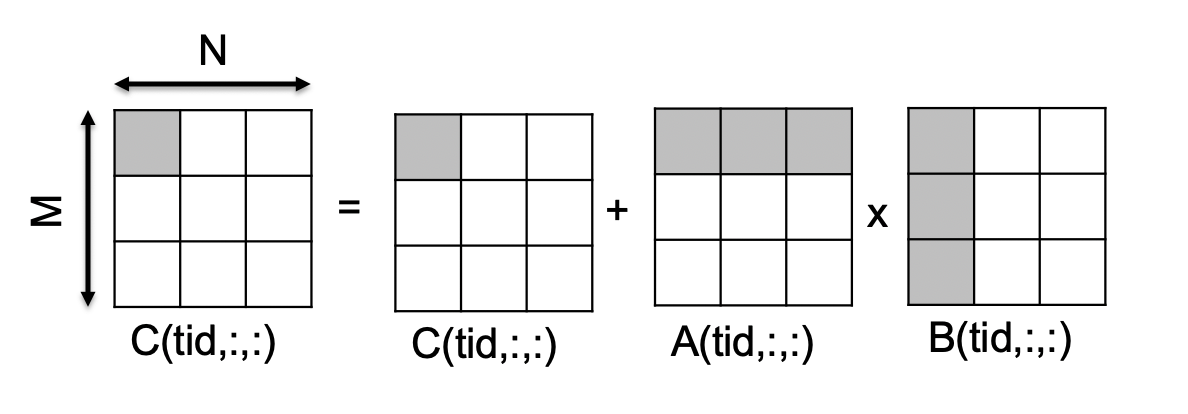
\includegraphics[width=0.65\textwidth]{figures/TeamGemm}
  \end{center}
  \vspace{-1em}
  \scriptsize{Related exercise available at: \verb!Exercises/kokkoskernels/TeamGemm!}
\end{frame}
%==========================================================================
\begin{frame}[fragile]{KokkosBatched interfaces - BlockJacobi}
  \Huge {Exercise: BlockJacobi}
\end{frame}

%==========================================================================
\begin{frame}[fragile]{KokkosBatched interfaces - BlockJacobi}

  \begin{itemize}
  \item Objective:
    \begin{itemize}
    \item \small{Compose a batched LU factorization of diagonal blocks and compute inverse of the blocks}
    \item \small{Compare a non-fused batched functions against the fused batch function using functor level interface} 
    \end{itemize}
  \item Exercise: \url{https://github.com/kokkos/kokkos-tutorials/tree/main/Exercises/kokkoskernels/BlockJacobi/Begin}
  \item On GPUs,
    \begin{itemize}
    \item Test the code with different team size \verb|run-different-teamsize.sh|
    \item Profile the code using nvprof \verb|run-nvprof.sh|
    \end{itemize}
  \end{itemize}

\end{frame}

%==========================================================================
\begin{frame}[fragile]{KokkosBatched interfaces - BlockJacobi}

  \begin{itemize}
  \item \small{\url{Exercises/kokkoskernels/BlockJacobi/Solution/run-different-teamsize.sh}}
  \item \small{This inverts 16,384 instances of 5x5 block matrices}
    \begin{tabular}{ccc}
      \hline
      \quad & \multicolumn{2}{c}{\# of inversion per sec} \\
      TeamSize & Non-fused & Fused \\
      \hline
      AUTO & 3,385 & \textbf<2>{5,054} \\
      32   & \textbf<3>{4,603} & \textbf<1,2,3>{8,766} \\
      64   & 4,199 & 6,488 \\
      96   & 3,581 & 5,017 \\
      \hline
    \end{tabular}
  \item Why 32 TeamSize is the best ?
    \begin{itemize}
    \item \footnotesize{For simplicity, assuming 25 entries of a block matrix are updated independently, 25 is the maximum team size}
    \item \footnotesize{By fusing multiple operations, temporal locality is exploited}
    \item \footnotesize{Need to check this using a profiler, nvprof}
    \end{itemize}
  \item \small{\url{Exercises/kokkoskernels/BlockJacobi/Solution/run-nvprof.sh}}
    \begin{itemize}
    \item<2-3> \only<2>{Comparison 1, AUTO vs 32} \only<3>{Comparison 2, non-fused vs fused}
    \end{itemize}
  \end{itemize}
  
\end{frame}

\begin{frame}[fragile]{KokkosBatched interfaces - BlockJacobi}

  Comparison 1: the same code with different team size
  \begin{itemize}
  \item \footnotesize{AUTO (set TeamSize = 96) shows higher occupancy}
    \begin{center}
      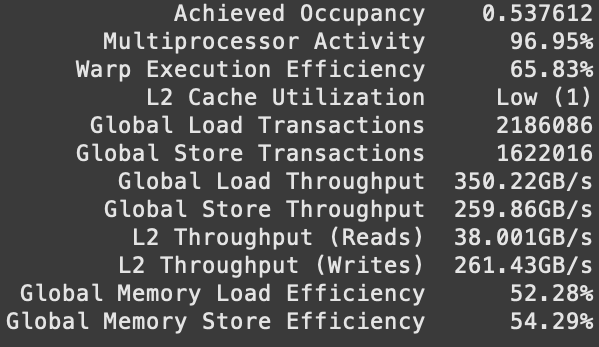
\includegraphics[width=0.40\textwidth]{figures/BATCHED-blockjacobi-auto-fused.png}
    \end{center}
  \item \footnotesize{TeamSize = 32 leads higher global load/store throughput, resulting 1.7x speedup }
    \begin{center}
      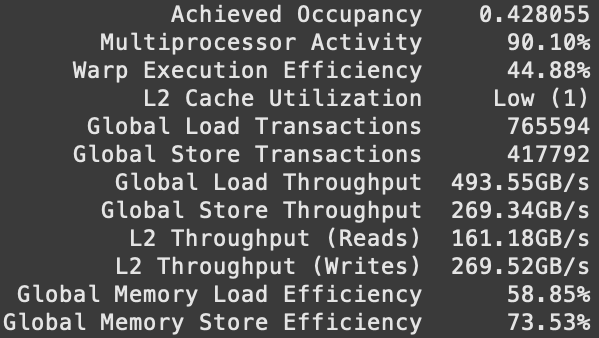
\includegraphics[width=0.40\textwidth]{figures/BATCHED-blockjacobi-team32-fused.png}
    \end{center}
  \end{itemize}

\end{frame}

\begin{frame}[fragile]{KokkosBatched interfaces - BlockJacobi}

  Comparison 2: the same code with non-fused vs fused version
  \begin{itemize}
  \item \footnotesize{For non-fused version, we show one best performing kernel of four kernels}
    \begin{center}
      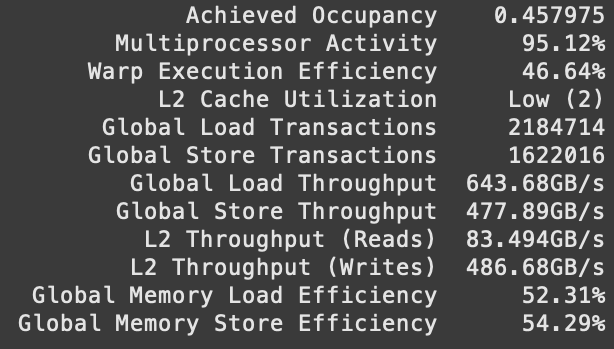
\includegraphics[width=0.40\textwidth]{figures/BATCHED-blockjacobi-team32-nonfused.png}
    \end{center}
  \item \footnotesize{Fused version performs 1.9x faster than non-fused version}
    \begin{center}
      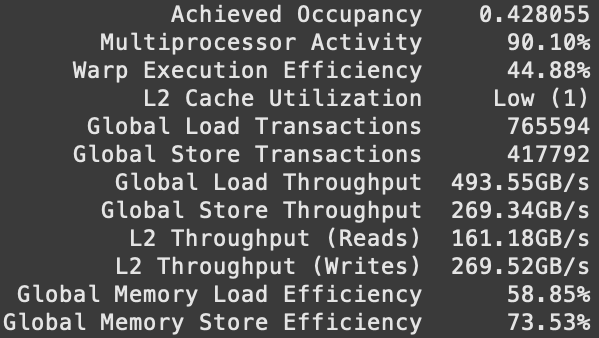
\includegraphics[width=0.40\textwidth]{figures/BATCHED-blockjacobi-team32-fused.png}
    \end{center}
  \item \footnotesize{Note that non-fused interface can be optimized much better for each kernel and specific problem size}
  \end{itemize}

\end{frame}

\begin{frame}[fragile]{Summary}

  \textbf{Summary: Batched BLAS/LAPACK}
  \begin{itemize}
  \item \small{User composable batched interface: parallel execution policy + functor-level interface}
  \item \small{Performance on GPUs is tunable:}
    \begin{itemize}
    \item \small{Launching light-weight kernels multiple times can cause overhead}
    \item \small{Fusing too many functor-level BLAS/LAPACK operations is difficult to perform optimal with a single team size}
    \end{itemize}
  \end{itemize}
  
\end{frame}

\begin{frame}[fragile]

  {\Huge Sparse Linear Algebra}

  \vspace{10pt}

  {\large Sparse linear algebra data structures and functions.}

  \vspace{20pt}

  \textbf{Learning objectives:}
  \begin{itemize}
    \item {Key characteristics algorithms}
    \item {Containers: CrsMatrix, StaticCrsGraph, Vector}
    \item {SpMV}
    \item {SpADD}
    \item {SpGEMM}
  \end{itemize}

  \vspace{-20pt}

\end{frame}

%==========================================================================

\begin{frame}[fragile]{Why do we need this?}
  \textbf{Support for important class of applications}

  \begin{itemize}
  \item Representation of choices for discrete PDE systems (FEM, FD, CVFEM, ...)
  \item Natural use for network representation
    \begin{itemize}
    \item Electrical grid, electronic circuit
    \item Social network
    \end{itemize}
  \end{itemize}


  \begin{block}{Unique format supported: Compressed row sparse}
    Sparse matrices can be stored in various format, currently only Crs format is fully supported, BlockCrs is partially supported
  \end{block}
\end{frame}

\begin{frame}[fragile]{Algorithmic characteristics}
\textbf{Constraints from Crs format}

\begin{itemize}
\item hard to optimize memory access patterns
\item often multi-pass algorithms required
  \begin{enumerate}
  \item compute storage
  \item compute column index and actual values
  \end{enumerate}
\item typically algorithms can be split in symbolic and numeric phases
\end{itemize}

\begin{block}{Symbolic/Numeric split}
  While extremely useful for reuse it is potentially slower for single use case depending on implementation
\end{block}
\end{frame}

\begin{frame}[fragile]{KokkosKernels Handle}
\textbf{Handle: hiding important details!}

\begin{itemize}
\item What the handles does for you:
  \begin{itemize}
  \item stores user parameters
  \item keeps temporary data needed in numeric of solve/apply phases
  \item cleans up temporary data at destruction
  \item contains kernel specific "sub-handle"
  \item specifies required data types
  \end{itemize}

\item Usage: \texttt{KokkosKernels::Experimental::\\ KokkosKernelsHandle<size\_type,\\
  \hspace{3.8cm} index\_type,\\
  \hspace{3.8cm} scalar\_type,\\
  \hspace{3.8cm} ExecutionSpace,\\
  \hspace{3.8cm} TempMemSpace,\\
  \hspace{3.8cm} PermMemSpace>()}
\end{itemize}
\end{frame}

\begin{frame}[fragile]{Containers}

\textbf{One dense structure:}
\begin{itemize}
\item \texttt{View} (of rank 1): represents a "vector"
\item \texttt{View} (of rank 2): represents a "multi-vector"
\end{itemize}

\vspace{1em}
\textbf{Two sparse structures:}
\begin{itemize}
  \item \texttt{StaticCrsGraph}: encodes the sparsity pattern in \texttt{row\_map} and \texttt{entries}
  \item \texttt{CrsMatrix}: contains a \texttt{StaticCrsGraph} and \texttt{values}
\end{itemize}

\vspace{1em}
\textbf{Example:}
\texttt{example/wiki/sparse/KokkosSparse\_wiki\_crsmatrix.cpp}
\end{frame}

\begin{frame}{Sparse kernels interfaces}
  \textbf{Two interfaces for one kernel?}
  \begin{enumerate}
  \item Simplified interface
    \begin{itemize}
    \item uses high level containers
    \item reduced number of parameters and templates
    \item allocates memory
    \end{itemize}
  \item Expert interface
    \begin{itemize}
    \item uses low level container (i.e. views)
    \item allows for finer memory management
    \end{itemize}
  \end{enumerate}

\begin{block}{Simplified/Expert interface}
  For clarity we will focus on the simplified interface in the rest of the lecture
\end{block}
\end{frame}

\begin{frame}[fragile]{SpMV}
  \textbf{SpMV: a mixed sparse/dense kernel}

  \begin{equation*}
  0.5*\begin{bmatrix}
    4\\ 5\\ 6\\
  \end{bmatrix}+1.0
  \begin{bmatrix}
    1 & & 2 \\
    & 3 & \\
    4 & & 5 \\
  \end{bmatrix}
  \begin{bmatrix}
    1\\ 2\\ 3\\
  \end{bmatrix}
  =\begin{bmatrix}
  9 \\ 8.5 \\ 22
  \end{bmatrix}
  \end{equation*}
  
  \begin{itemize}
  \item Computes: $y = \beta*y + \alpha*A*x$
  \item Output is a dense vector
    \begin{itemize}
    \item single pass algorithm since no CrsGraph needs to be computed
    \item good amount of parallelism exploitable
    \end{itemize}
  \item Usage:  \\ \hspace{1em}\texttt{KokkosSparse::spmv(mode, alpha, A, x, beta, y);}
  \item Example:\\ \hspace{1em}\texttt{example/wiki/sparse/KokkosSparse\_wiki\_spmv.cpp}
  \end{itemize}
\end{frame}

\begin{frame}[fragile]{SpADD}
  \textbf{SpADD: Sparse Matrix Addition}
    \begin{equation*}
      2.0\begin{bmatrix}
        1 &   & 2 \\
          & 3 & 4 \\
        5 &   &   \\
      \end{bmatrix}
      +0.5\begin{bmatrix}
      6 &  7 &  \\
        &  8 &  \\
        &    & 9\\
      \end{bmatrix}
      =\begin{bmatrix}
       5 & 3.5 &   4\\
         &  10 &   8\\
      10 &     & 4.5\\
      \end{bmatrix}
    \end{equation*}
  
  \begin{itemize}
  \item Computes: $C=\alpha A + \beta B$ given $A$ and $B$ two CrsMatrices
  \item Sorted inputs speeds-up the kernel and reduces memory consumption
  \item Usage:\\
    \hspace{1em} \texttt{KokkosSparse::spadd\_symbolic(handle, A, B, C);}\\
    \hspace{1em} \texttt{KokkosSparse::spadd\_numeric(handle, alpha, A, beta, B, C);}
  \item Example:\\
    \hspace{1em} \texttt{example/wiki/sparse/KokkosSparse\_wiki\_spadd.cpp}
  \end{itemize}
\end{frame}


\begin{frame}[fragile]{SpGEMM}
\textbf{SpGEMM: Sparse General Matrix Matrix Multiply}
 
\vspace{.4cm}

\begin{itemize}

  \item Compute $A\times B=C$ for given sparse matrices $A$ and $B$
  \begin{equation*}
  \left[ 
  \begin{tabular}{ccc}
	1 &    & 2 \\
   	   & 3 & 4 \\
        5 &    & 
  \end{tabular}
  \right]
  \times
  \left[ 
  \begin{tabular}{r r r r}
	6 &    & 7 & \\
   	8 & 9 &    & \\
           &    &10&11 
  \end{tabular}
  \right] 
  =
    \left[ 
  \begin{tabular}{r r r r}
	  6 &      & 27 & 22 \\
   	24 & 27 & 40 & 41 \\
        30 & 35 &      &      \\ 
  \end{tabular}
  \right]   
\end{equation*}
  \begin{itemize}
     \item Sparsity structure of $C$ is not known in advance!
  \end{itemize}
  
  \vspace{.4cm}
  
  \item We have a two-phase implementation:
  \begin{itemize}
    \item This allows determining the sparsity of $C$ efficiently
  \end{itemize}
 \end{itemize}  
\end{frame}

\begin{frame}[fragile]{SpGEMM}
\textbf{SpGEMM: Sparse General Matrix Matrix Multiply}

\vspace{.4cm}

\begin{itemize}
\item \textbf{Symbolic phase:} 
  \begin{itemize} 
  \item \texttt{KokkosSparse::spgemm\_symbolic(handle, \\ 
    \hspace{2.9cm}A, isTrnspsdA, B, isTrnspsdB, C);} 
  \item determines number of nonzeros in each row of $C$ and
  \item allocates memory for column indices and values of the nonzeros
  \end{itemize} 

  \vspace{.4cm}

\item \textbf{Numeric phase}
  \begin{itemize}
  \item \texttt{KokkosSparse::spgemm\_numeric(handle, \\ 
    \hspace{2.7cm}A, isTrnspsdA, B, isTrnspsdB, C);}
  \item computes column indices and values of the nonzeros of $C$
  \end{itemize}

  \vspace{.4cm}

\item \textbf{Example}\\[-3ex]
  \hspace{1em} \texttt{example/wiki/sparse/KokkosSparse\_wiki\_spgemm.cpp}
\end{itemize}  
\end{frame}


\begin{frame}[fragile]{SpGEMM}
\textbf{SpGEMM: Sparse General Matrix Matrix Multiply}

\begin{itemize}

  \item We follow Gustavson's algorithm: \\
   \hspace{0.4cm}   \textbf{for} each row index $i\gets 0$  \textbf{to} $nrowsA$ \textbf{do} \\
   \hspace{0.8cm} 	   \textbf{for} each column index $j\in A(i,:)$ \textbf{do} \\
   \hspace{1.2cm}	     	//\texttt{accumulate partial row results}\\
   \hspace{1.2cm}	     	$C(i,:) \gets C(i,:) + A(i,j)B(j,:)$
   
  \vspace{.4cm}
  \item Our implementation exploits hierarchical paralelism
  \begin{itemize}
  	\item Teams are assigned contiguous row chunks in $A$  
      	\item Threads are assigned individual rows of $A$
        \item Vector lanes are assigned the nonzeros of rows of $B$
  \end{itemize} 


 \end{itemize}  
\end{frame}

\begin{frame}[fragile]{SpGEMM}
\textbf{SpGEMM: Sparse General Matrix Matrix Multiply}

\begin{itemize}
  \item We follow Gustavson's algorithm: \\
   \hspace{0.4cm}   \textbf{for} each row index $i\gets 0$  \textbf{to} $nrowsA$ \textbf{do} \\
   \hspace{0.8cm} 	   \textbf{for} each column index $j\in A(i,:)$ \textbf{do} \\
   \hspace{1.2cm}	     	//\texttt{accumulate partial row results}\\
   \hspace{1.2cm}	     	$C(i,:) \gets C(i,:) + A(i,j)B(j,:)$
  \item Our thread-scalable hashmap accumulator implementation
  \begin{itemize} 
    	\item is used in both symbolic and numeric phases
  	\item supports both sparse and dense accumulators
	\item has a two-level structure: Level-1 ($L_1$) and Level-2 ($L_2$)
	\begin{itemize}
	  \item $L_1$ hashmap lives in the fast shared memory
	  \item $L_2$ hashmap is created only if $L_1$ hashmap runs out of memory
	  \item $L_2$ hashmap lives in the large global memory 
	\end{itemize}
  \end{itemize}
  \item For more details see: {\footnotesize M. Deveci, C. Trott, S. Rajamanickam, "Multithreaded sparse matrix-matrix multiplication for many-core and GPU architectures", Parallel Computing 78, 33-46, 2018.}
 \end{itemize}  
\end{frame}

\begin{frame}[fragile]{Summary SpLA}

  \textbf{Summary: Sparse Linear Algebra}
  \begin{itemize}
    \item {Main difficulties: finding sparsity patterns and memory access}
    \item {Containers: \texttt{View}, \texttt{StaticCrsGraph} and \texttt{CrsMatrix}}
    \item {Kernels: SpMV, SpADD and SpGEMM}
  \end{itemize}

\end{frame}

\begin{frame}[fragile]

  {\Huge Graph Kernels}

  \vspace{10pt}

  {\large Kokkos Kernels functionality for graph computations.}

  \vspace{20pt}

  \textbf{Learning objectives:}
  \begin{itemize}
    \item {Distance-1 Graph Coloring}
    \item {Distance-2 Graph Coloring}
    \item {Bipartite Graph Partial Coloring}
  \end{itemize}

  \vspace{-20pt}

\end{frame}

%==========================================================================

\begin{frame}[fragile]{Distance-1 Coloring}

\textbf{Distance-1 Graph Coloring}

\begin{itemize}
  \item Given a graph, assign a color to each vertex so that no two adjacent vertices have the same color
  \item Minimizing the number of unique colors is NP-hard
  \item Approximate solution (with a few more colors than optimal) is still useful
  \item KokkosKernels has two main algorithms for this: vertex-based and edge-based
\end{itemize}
\end{frame}

\begin{frame}[fragile]{Distance-1 Graph Coloring}
\textbf{Vertex-Based (VB) Coloring}

Initialize worklist containing every vertex.
\begin{itemize}
  \item In parallel, for each vertex v in worklist:
  \begin{itemize}
    \item Assign smallest color to v which isn't found on any neighbor
  \end{itemize}
  \item In parallel, for each vertex v in worklist:
  \begin{itemize}
    \item If v's color is matches with a neighbor, uncolor v and add it to next worklist
  \end{itemize}
\end{itemize}
These steps are repeated until the worklist is empty (all vertices have been colored).
\end{frame}

\begin{frame}[fragile]{Distance-1 Graph Coloring}
\textbf{Edge-Based (EB) Coloring}

Initialize worklist containing every edge.
\begin{itemize}
  \item In parallel, for each edge e in worklist:
  \begin{itemize}
    \item If both endpoints of e have the same color, uncolor the one with a higher ID
    \item If at least one endpoint of e is uncolored, add e to the next worklist.
  \end{itemize}
  \item In parallel, for each edge e in worklist:
  \begin{itemize}
    \item If exactly one endpoint is colored, add that color to forbidden set for other endpoint
  \end{itemize}
  \item In parallel, for each uncolored vertex v:
  \begin{itemize}
    \item Color v with smallest non-forbidden color
  \end{itemize}
\end{itemize}
These steps are repeated until the edge worklist is empty, meaning both endpoints of every edge have been colored.
\end{frame}

\begin{frame}[fragile]{Distance-1 Graph Coloring}
\textbf{Algorithm Summary}

\begin{itemize}
  \item EB pseudocode was simplified, did not include tentative coloring (technique for faster convergence)
  \item In VB, work per thread requires loop over neighbors of a vertex
  \item In EB, work per thread is constant time, but the worklists are longer
  \item EB is significantly faster on GPUs when the maximum degree is high (generally, $> 3000$)
  \item Otherwise, VBBIT (VB with bitwise operations to track forbidden colors) is usually the fastest.
  \item Use enum values \verb!KokkosGraph::COLORING_VBBIT! and \verb!KokkosGraph::COLORING_EB! 
\end{itemize}
\end{frame}

\begin{frame}[fragile]{Distance-1 Graph Coloring}
\textbf{Using Distance-1 Coloring}

\begin{code}
  #include "KokkosGraph_Distance1Color.hpp"
  KokkosKernels::KokkosKernelsHandle<...> handle;
  // Choose algorithm and set up
  handle.create_graph_coloring_handle(KokkosGraph::COLORING_VB);
  // Compute the coloring
  KokkosGraph::Experimental::graph_color(&handle,
    numVertices, numVertices, rowmap, entries);
  // Get the subhandle for coloring
  auto colorHandle = handle.get_graph_coloring_handle();
  // Get the number of colors used, and color labels
  auto numColors = colorHandle->get_num_colors();
  auto colors = colorHandle->get_vertex_colors();
  // Clean up
  handle.destroy_graph_coloring_handle();
\end{code}
\end{frame}

\begin{frame}[fragile]{Distance-2 Coloring and BGPC}
\textbf{Distance-2 Coloring Problem}

\begin{itemize}
  \item Each vertex must have a different color than all vertices within 2 hops of it
  \item If $G$ is represented by adjacency matrix, this is equivalent to computing distance-1 coloring on $G^2$
  \item Graph must be undirected (symmetric adjacency matrix)
\end{itemize}
\end{frame}

\begin{frame}[fragile]{Distance-2 Coloring and BGPC}
\textbf{Distance-2 Coloring Problem}

In this graph, 0 couldn't have the same color as 1 or 2, but it could have the same as 3 or 4.
\begin{figure}[h]
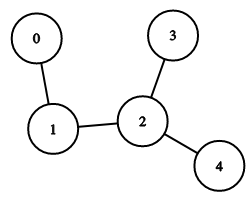
\includegraphics[width=0.5\textwidth]{figures/dist2_graph_example}
\end{figure}
\end{frame}

\begin{frame}[fragile]{Distance-2 Coloring and BGPC}
\textbf{Bipartite Graph Partial Coloring}

\begin{itemize}
  \item Closely related to distance-2 coloring
  \item Color either left or right side of a bipartite graph so that any vertices 2 hops apart have different colors
  \item Left-side BGPC equivalent to distance-1 coloring on $GG^\top$
  \item Right-side BGPC equivalent to distance-1 coloring on $G^{\top}G$
\end{itemize}
\end{frame}

\begin{frame}[fragile]{Distance-2 Coloring and BGPC}
\textbf{Bipartite Graph Partial Coloring}
\begin{itemize}
  \item For left-sided coloring of this graph, 1 couldn't have the same color as 0, but could have the same as 2.
  \item For right-sided coloring of this graph, vertices 3, 4 and 5 must all have different colors.
\end{itemize}
\begin{figure}[h]
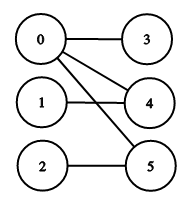
\includegraphics[width=0.4\textwidth]{figures/bgpc_example}
\end{figure}
\end{frame}

\begin{frame}[fragile]{Distance-2 Coloring and BGPC}
\textbf{D2/BGPC Algorithms}
\begin{itemize}
  \item VB (\verb!KokkosGraph::COLORING_D2_VB_BIT!): Just like distance-1 VB, but coloring and conflict resolution loop over neighbors-of-neighbors, not just neighbors
  \item NB (\verb!KokkosGraph::COLORING_D2_NB_BIT!) Net-based coloring from ``Greed is Good: Parallel Algorithms for BGPC'' by Ta\c{s} et al.
    Is asymptotically faster than VB by avoiding neighbors-of-neighbors loops, and is faster in practice.
\end{itemize}
\end{frame}

\begin{frame}[fragile]{Distance-2 Coloring and BGPC}
\textbf{Using Distance-2 Coloring}

\begin{code}
  #include "KokkosGraph_Distance2Color.hpp"
  KokkosKernels::KokkosKernelsHandle<...> handle;
  // Set up for coloring, and choose algorithm
  handle.create_distance2_graph_coloring_handle(
    KokkosGraph::COLORING_D2_NB_BIT);
  // Compute the coloring
  KokkosGraph::Experimental::graph_color_distance2(
    &handle, numVertices, rowmap, entries);
  // Get the subhandle for D2 coloring
  auto colorHandle =
    handle.get_distance2_graph_coloring_handle();
  auto numColors = colorHandle->get_num_colors();
  auto colors = colorHandle->get_vertex_colors();
  handle.destroy_distance2_graph_coloring_handle();
\end{code}
\end{frame}

\begin{frame}[fragile]{Distance-2 Coloring and BGPC}
\textbf{Using BGPC} 

Same handle and algorithm choices as D2, but use:
\begin{code}
KokkosGraph::Experimental::bipartite_color_rows(
  &handle, numRows, numColumns, rowmap, entries);
\end{code}

and:

\begin{code}
KokkosGraph::Experimental::bipartite_color_columns(
  &handle, numRows, numColumns, rowmap, entries);
\end{code}
\end{frame}

\begin{frame}[fragile]{Exercise}
\textbf{Coloring Exercise}
\begin{itemize}
  \item \verb!Intro-Full/Exercises/kokkoskernels/GraphColoring!
  \item Compute both D1 and D2 colorings of a graph
  \item The graph is generated as a 9-point stencil on a small 2D grid
  \item The colors will be printed out in the layout of the grid
\end{itemize}
\begin{figure}[h!]
  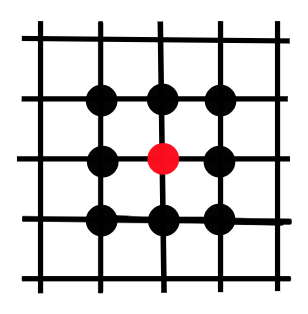
\includegraphics[width=0.3\textwidth]{figures/9pt_stencil.png}
  \caption{A 9-point stencil. The black points are adjacent to the red point.}
\end{figure}

\end{frame}

\begin{frame}[fragile]{Summary}
\textbf{Summary: Graph Algorithms}
\begin{itemize}
  \item Distance-1 Coloring
  \begin{itemize}
    \item vertex-based (VB) and edge-based (EB) based algorithms
    \item Use \verb!COLORING_VBBIT!, unless maximum degree $> 3000$ - then use \verb!COLORING_EB!
  \end{itemize}
  \item Distance-2 and Bipartite Graph Partial Coloring
  \begin{itemize}
    \item vertex-based (VB) and net-based (NB) algorithms
    \item Use \verb!COLORING_D2_NB_BIT! for best performance
  \end{itemize}
\end{itemize}

\end{frame}

\begin{frame}[fragile]

  {\Huge Sparse Solvers}

  \vspace{10pt}

  {\large Gauss-Seidel Preconditioners}

  \vspace{20pt}

  \textbf{Learning objectives:}
  \begin{itemize}
    \item {Multicolor Gauss-Seidel}
    \item {Cluster Gauss-Seidel}
    \item {Two-Stage Gauss-Seidel}
  \end{itemize}

  \vspace{-20pt}

\end{frame}

%==========================================================================

\begin{frame}[fragile]{Multicolor Gauss-Seidel}
\textbf{Multicolor Gauss-Seidel}

Gauss-Seidel (GS) method for solving $A\mathbf{x} = \mathbf{b}$ updates one entry of the unknown at a time:

For $i = 1..M$:
\[ \mathbf{x}_i := (\mathbf{b}_i - \sum_{j=1}^{N} A_{ij}\mathbf{x}_j) / A_{ii}\]

\begin{itemize}
  \item Standard GS is sequential: updates to $\mathbf{x}_i$ are affected by previous updates to $\mathbf{x}_j$ in the same iteration (where $j < i$)
  \item Treating A as a graph's adjacency matrix, $A_{ij} \neq 0$ if vertices $i$ and $j$ are adjacent
  \item Suppose a coloring is computed for this graph, and $\mathit{Color}(i) = \mathit{Color}(j)$.
  \item then $\mathbf{x}_j$ does not directly affect the updated value of $\mathbf{x}_i$
\end{itemize}
\end{frame}

\begin{frame}[fragile]{Multicolor Gauss-Seidel}
\textbf{Using KokkosKernels Multicolor GS}

KokkosKernels supports preconditioning with multicolor GS. Rows with the same color are updated in parallel.

\begin{code}
  #include "KokkosSparse_gauss_seidel.hpp"
  // Handle creation
  KokkosKernels::KokkosKernelsHandle<...> handle;
  handle.create_gs_handle(KokkosSparse::GS_POINT);
  // Symbolic setup
  KokkosSparse::Experimental::gauss_seidel_symbolic(
    &handle, numRows, numCols,
    A.graph.row_map, A.graph.entries, graphIsSymmetric);
  // Numeric setup
  KokkosSparse::Experimental::gauss_seidel_numeric(
    &handle, numRows, numCols,
    A.graph.row_map, A.graph.entries, A.values,
    graphIsSymmetric);
\end{code}
\end{frame}

\begin{frame}[fragile]{Multicolor Gauss-Seidel}
\textbf{Using KokkosKernels Multicolor GS, continued}

KokkosKernels supports parallel preconditioning with multicolor GS.

\begin{code}
  KokkosSparse::Experimental::forward_sweep_gauss_seidel_apply(
    &handle, numRows, numCols,
    A.graph.row_map, A.graph.entries, A.values,
    x, b, initZeroX, updateCachedB, omega, numSweeps);
  // --- or ---
  KokkosSparse::Experimental::backward_sweep_gauss_seidel_apply(
    &handle, numRows, numCols,
    A.graph.row_map, A.graph.entries, A.values,
    x, b, initZeroX, updateCachedB, omega, numSweeps);
  // --- or ---
  KokkosSparse::Experimental::symmetric_gauss_seidel_apply(
    &handle, numRows, numCols,
    A.graph.row_map, A.graph.entries, A.values,
    x, b, initZeroX, updateCachedB, omega, numSweeps);
  // Clean up
  handle.destroy_gs_handle();
\end{code}
\end{frame}

\begin{frame}[fragile]{Multicolor Gauss-Seidel}
\textbf{Using KokkosKernels Multicolor GS}

\begin{itemize}
  \item Algorithm called \verb!POINT! because individual rows of the matrix are colored, as opposed to blocks/clusters
  \item \verb!graphIsSymmetric!: whether the matrix is structurally symmetric.
    If false, must symmetrize before coloring.
  \item \verb!initZeroX!: whether to zero out $\mathbf{x}$ before starting
  \item \verb!updateCachedB!: whether on the first apply, or $\mathbf{b}$ has changed since the last apply
  \item \verb!omega!: damping factor for successive over-relaxation (default is 1.0)
  \item \verb!numSweeps!: how many applications to perform. For symmetric apply, forward+back counts as 1 application.
\end{itemize}

\end{frame}

\begin{frame}[fragile]{Cluster Gauss-Seidel}
\textbf{Cluster GS}

\begin{itemize}
  \item In Multicolor GS, an independent row $j$ does not \emph{directly} affect the updated value of $\mathbf{x}_i$, but it can affect it \emph{indirectly}.
  \item For example, if $i$ and $j$ have the same color and are separated by $k$,
    then information is not transferred from $\mathbf{x}_i$ to $\mathbf{x}_j$ through $\mathbf{x}_k$ within a sweep.
  \item This is why multicolor GS usually gives a slightly worse answer than sequential GS.
  \item To help with this, cluster GS coarsens the graph and applies GS sequentially within a cluster.
\end{itemize}
\end{frame}

\begin{frame}[fragile]{Cluster Gauss-Seidel}
\textbf{Cluster GS}
Example:
\begin{code}
  handle.create_gs_handle(
    KokkosSparse::CLUSTER_BALLOON, clusterSize);
\end{code}
\begin{itemize}
  \item ``Balloon'' is the coarsening algorithm (others may be added in the future)
  \item \verb!clusterSize! is the coarsening factor (an integer larger than 1, but should be small compared to the number of rows)
  \item The symbolic, numeric and apply interface is the same as multicolor (\verb!POINT!)
\end{itemize}
\end{frame}

\begin{frame}[fragile]{Two-Stage Gauss-Seidel}
\textbf{Two-Stage GS}
\begin{itemize}
  \item Hybrid of the Jacobi and Gauss-Seidel methods
  \item Formulates Gauss-Seidel as a lower or upper triangular solve (for forward and backward sweeps, respectively),
    and uses some number of Jacobi sweeps as an approximation for this solve.
\end{itemize}

Usage:

\begin{code}
  handle.create_gs_handle(KokkosSparse::TWO_STAGE);
\end{code}
\end{frame}

\begin{frame}[fragile]{Exercise}
\textbf{GS: Exercise}
\begin{itemize}
  \item \verb!Intro-Full/Exercises/kokkoskernels/GaussSeidel!
  \item Generates a small, diagonally dominant system
  \item Fill in the neccesary calls to set up and use one of the GS algorithms as an iterative solver
\end{itemize}
\end{frame}

\begin{frame}[fragile]{Summary}
\textbf{Summary: Gauss-Seidel}
\begin{itemize}
  \item Multicolor Gauss-Seidel
  \begin{itemize}
    \item Uses coloring to find independent rows
  \end{itemize}
  \item Cluster Gauss-Seidel
  \begin{itemize}
    \item Like multicolor but coarsens graph first
  \end{itemize}
  \item Two-Stage Gauss-Seidel
  \begin{itemize}
    \item Hybrid Gauss-Seidel/Jacobi-Richardson
  \end{itemize}
\end{itemize}

The best choice depends on the problem.

\end{frame}

%==========================================================================

\begin{frame}[fragile]

  {\Huge Sparse Solvers 2}

  \vspace{10pt}

  {\large Sparse factorization and triangular solver.}

  \vspace{20pt}

  \textbf{Learning objectives:}
  \begin{itemize}
    \item {Sparse incomplete LU factorization}
    \item {Sparse triangular solvers}
  \end{itemize}

  \vspace{-20pt}

\end{frame}

%==========================================================================

\begin{frame}[fragile]{Overview}
\textbf{SPARSE SPILUK and SPTRSV}

KokkosKernels supports preconditioning with sparse incomplete LU factorization coupled with sparse triangular solvers.

%\[ A\mathbf{x} = b \Leftrightarrow M^{-1}A\mathbf{x} = M^{-1}\mathbf{b} \]

\begin{itemize}
%  \item Use case: ILU to generate LU factorization for preconditioner used with linear iterative solvers, robust for elliptic PDE's, does not work well for indefinite systems
  \item \textbf{SPILUK}: Sparse k-level incomplete LU factorization
  \begin{itemize}
    \item Computes sparse lower triangular matrix $L$ and upper triangular matrix $U$ such that $M = LU$ is "similar" to $A$
    \item $k = 0$: No additional fill-in. $G(L+U) = G(A)$
    \item $k > 0$: Increased fill level improves accuracy
  \end{itemize}
  \vspace{1em}
  \item \textbf{SPTRSV}: Sparse triangular solver
  \begin{itemize}
    \item Apply ILU: $\mathbf{z} = M^{-1}\mathbf{r} \Leftrightarrow z = (LU)^{-1}\mathbf{r} \Leftrightarrow z = U^{-1}(L^{-1}\mathbf{r})$
    \item L,U reused by triangular solver to apply preconditioning during linear solver iterations
  \end{itemize}
\end{itemize}

\end{frame}

\begin{frame}[fragile]{SPILUK}
\textbf{SPILUK usage}

  \begin{itemize}
    \item ILU(k): requires matrices in "Crs" format
    \item Symbolic phase on host (serial):
    \begin{itemize}
      \item Construct nonzero patterns of L and U
      \item Perform level-scheduling to group independent rows into levels based on L's sparsity pattern. Level-scheduling results stored within a handle for reuse
    \end{itemize}
    \item Numeric phase (parallel) fill data to the nonzero patterns based on level-scheduling results found in the symbolic phase
    \item Algorithm options:
    \begin{itemize}
      \item SEQLVLSCHD\_RP: using range policy parallelism for numeric phase
      \item SEQLVLSCHD\_TP1: using team policy parallelism for numeric phase
    \end{itemize}
  \end{itemize}

\end{frame}

\begin{frame}[fragile]{SPILUK}
\textbf{SPILUK: Interface}

  \begin{itemize}
    \item \{A,L,U\}\_rowmap: Arrays storing row pointer offset, as a 1-D Kokkos::View
    \item \{A,L,U\}\_entries: Arrays storing column indices, as a 1-D Kokkos::View
    \item \{A,L,U\}\_values: Arrays storing corresponding matrix values, as a 1-D Kokkos::View
    \item Handle: Stores internal data structures from symbolic phase
    \begin{itemize}
      \item Input: SPILUKAlgorithm, number of rows, est. number of nonzeros L, est. number of nonzeros of U
      \item Templated on rowmap data type (size\_type), entries ordinal type (lno\_t), values scalar type (scalar\_t), execution space, "persistent" memory space, "temporary" memory space (unused here)
    \end{itemize}
  \end{itemize}

\end{frame}

\begin{frame}[fragile]{SPILUK}
\textbf{SPILUK: Interface}

\begin{itemize}
  \item<2-> Include header file
    \begin{code}[keywords={parallel_reduce,for,int,double}, basicstyle=\tiny, breaklines=true]
#include "KokkosSparse_spiluk.hpp"
  //SPILUK in Experimental namespace - interface may evolve
using namespace KokkosKernels::Experimental;
    \end{code}

  \item<3-> Create opaque handle
    \begin{code}[keywords={parallel_reduce,for,int,double}, basicstyle=\tiny, breaklines=true]
KokkosKernelsHandle 
<size_type, lno_t, scalar_t, exec_space, mem_space, mem_space> kh;
    \end{code}

  \item<4-> Create the spiluk handle - requires estimate for nnz of L, U
    \begin{code}[keywords={parallel_reduce,for,int,double}, basicstyle=\tiny, breaklines=true]
nnzL = nnzU = EXPAND_FACT*A.nnz()*(fill_lev+1); // EXPAND_FACT set by user
kh.create_spiluk_handle(SPILUKAlgorithm, nrows, nnzL, nnzU);
    \end{code}

  \item<5-> Call symbolic routine
    \begin{code}[keywords={parallel_reduce,for,int,double}, basicstyle=\tiny, breaklines=true]
spiluk_symbolic(&kh, fill_level, A_rowmap, A_entries, 
                    L_rowmap, L_entries, U_rowmap, U_entries);
    \end{code}

  \item<6-> Call numeric routine
    \begin{code}[keywords={parallel_reduce,for,int,double}, basicstyle=\tiny, breaklines=true]
spiluk_numeric(&kh, fill_level, A_rowmap, A_entries, A_values, 
                                L_rowmap, L_entries, L_values, 
                                U_rowmap, U_entries, U_values);
    \end{code}

\end{itemize}

\end{frame}


\begin{frame}[fragile]{SPTRSV}
\textbf{SPTRSV usage}

  \begin{itemize}
    \item Sparse triangular solver: $\{L,U\}\mathbf{x} = \mathbf{b}$
    \begin{itemize}
      \item Fallback solver options
      \item Supernode-based solver options
    \end{itemize}
    \item Fallback implementation and TPL options:
    \begin{itemize}
      \item Symbolic phase analyzes matrix structure
      \begin{itemize}
        \item Level-scheduling employed to expose parallelism to solver
        \item All rows within a level can be solved independently in parallel
        \item Symbolic phase results stored within handle for reuse
      \end{itemize}
      \item Solve phase: Uses level-set information from symbolic to execute in parallel
      \item Separate phases allows reuse of symbolic phase / level scheduling information
      \begin{itemize}
        \item Use case: As direct solver for preconditioner for iterative solver methods, following factorization
      \end{itemize}
    \end{itemize}
  \end{itemize}

\end{frame}


\begin{frame}[fragile]{SPTRSV}
\textbf{SPTRSV usage}

  \begin{itemize}
      \item Algorithm options:
      \begin{itemize}
        \item SEQLVLSCHD\_TP1: Seq. level scheduling, solver hierarchical parallelism
        \item SEQLVLSCHD\_TP1CHAIN: Seq. level scheduling, solver hierarchical parallelism
        \begin{itemize}
          \item "Chaining" of consecutive levels with few rows into single kernel launch
          \item Reduces number of kernel launches for levels bound by launch overhead, e.g. banded matrices
        \end{itemize}
        \item SPTRSV\_CUSPARSE: Wrapper of NVIDIA's CuSPARSE triangular solver
      \end{itemize}
  \end{itemize}

\end{frame}


\begin{frame}[fragile]{SPTRSV}
\textbf{SPTRSV: Interface}
  \begin{itemize}
    \item \{L,U\}\_rowmap: Arrays storing row pointer offset, as a 1-D Kokkos::View
    \item \{L,U\}\_entries: Arrays storing column indices, as a 1-D Kokkos::View
    \item \{L,U\}\_values: Arrays storing corresponding matrix values, as a 1-D Kokkos::View
    \item Handle: Stores internal data structures from symbolic phase
    \begin{itemize}
      \item Input: SPTRSVAlgorithm, number of rows, boolean (is lower triangular)
      \item Templated on rowmap data type (size\_type), entries ordinal type (lno\_t), values scalar type (scalar\_t), execution space, "persistent" memory space, "temporary" memory space (unused here)
    \end{itemize}
    \item \{x,b\}: Dense vectors as rank-1 Views
  \end{itemize}

\end{frame}


\begin{frame}[fragile]{SPTRSV}
\textbf{SPTRSV: Interface}

\begin{itemize}
  \item<2-> Include header file
  \begin{code}[keywords={parallel_reduce,for,int,double}, basicstyle=\tiny, breaklines=true]
#include "KokkosSparse_sptrsv.hpp"
//SPTRSV in Experimental namespace - interface may evolve
using namespace KokkosKernels::Experimental;
  \end{code}

  \item<3-> Create opaque handle
  \begin{code}[keywords={parallel_reduce,for,int,double}, basicstyle=\tiny, breaklines=true]
KokkosKernelsHandle 
<size_t, lno_t, scalar_t, exec_sp, mem_sp, mem_sp> kh;
  \end{code}

  \item<4-> Create sptrsv handle - separate handles required for L and U
  \begin{code}[keywords={parallel_reduce,for,int,double}, basicstyle=\tiny, breaklines=true]
kh.create_sptrsv_handle(SPTRSVAlgorithm, nrows, lower_tri);
  \end{code}

  \item<5-> Call symbolic analysis
  \begin{code}[keywords={parallel_reduce,for,int,double}, basicstyle=\tiny, breaklines=true]
sptrsv_symbolic(&kh, rowmap, entries, values);
  \end{code}

  \item<6-> Call solve
  \begin{code}[keywords={parallel_reduce,for,int,double}, basicstyle=\tiny, breaklines=true]
sptrsv_solve((&kh, rowmap, entries, values, b, x);
  \end{code}
\end{itemize}
\end{frame}

%%%%%

\begin{frame}[fragile]{SPTRSV supernode-based}
\textbf{SPTRSV supernode-based usage}

  \begin{itemize}
      \item Users responsible for reordering and factorization to provide supernode block info
      \item Metis and SUPERLU software was used for this during development of the algorithm
      \item Symbolic phase analyzes matrix structure
      \begin{itemize}
        \item Level-set scheduling of supernode blocks
        \item Internal data structures are setup to store blocks
        \item Symbolic phase results stored within handle for reuse
        \item Optional: Merge supernodes with matching sparsity pattern
      \end{itemize}
      \item Compute phase
      \begin{itemize}
        \item Copy triangular matrix data to internal data structures
        \item Optional: Invert diagonal blocks; apply inverse to off-diagonal blocks
      \end{itemize}
      \item Solve phase: Uses level-set information to execute in parallel
      \item Separate phases allows reuse of symbolic and compute
  \end{itemize}

\end{frame}


\begin{frame}[fragile]{SPTRSV supernode-based}
\textbf{SPTRSV supernode-based usage}

  \begin{itemize}
%    \item Use cases:
%      \begin{itemize}
%        \item Domain-decomposition based linear solvers relying on direct solver for local solution
%        \item Multi-grid preconditioners with local sptrsv for coarse grid solve
%      \end{itemize}
    \item Algorithm options:
    \begin{itemize}
      \item SUPERNODAL\_DAG: Applies batched TRSV/GEMV kernels to supernodes at each level, internally computes DAG for scheduling
      \item SUPERNODAL\_SPMV\_DAG: Applies SPMV at each level and requires inverted diagonal blocks, internally computes DAG for scheduling
      \item SUPERNODAL\_ETREE: Like SUPERNODAL\_DAG, scheduling based on user-provided etree (e.g. from SuperLU)
      \item SUPERNODAL\_SPMV: Like SUPERNODAL\_SMPV\_DAG, scheduling based on user-provided etree
    \end{itemize}
    \item For more details see: \scriptsize{I. Yamazaki, S. Rajamanicakm, N. Ellingwood “Performance Portable Supernode-based Sparse Triangular Solver for Manycore Architectures”, \url{https://dl.acm.org/doi/fullHtml/10.1145/3404397.3404428}}
  \end{itemize}

\end{frame}

\begin{frame}[fragile]{SPTRSV supernode-based}
\textbf{SPTRSV: Interface supernode-based}

  \begin{itemize}
    \item \{L,U\}.graph: StaticCrsGraph data structure containing rowmap offsets and column indices
    \item nsuper: Number of supernode blocks
    \item supercols: Array of supernode block sizes
    \item etree: (Optional) Used for level scheduling
    \item Handle: Stores internal data structures and matrix blocks from symbolic and compute
    \begin{itemize}
      \item Input: SPTRSVAlgorithm, number of rows, boolean (is lower triangular)
      \item Templated on rowmap data type (size\_type), entries ordinal type (lno\_t), values scalar type (scalar\_t), execution space, "persistent" memory space, "temporary" memory space (unused here)
    \end{itemize}
    \item \{x,b\}: Dense vectors as rank-1 Views
  \end{itemize}
\end{frame}

\begin{frame}[fragile]{SPTRSV supernode-based}
\textbf{SPTRSV: Interface supernode-based}

\begin{itemize}
  \item<2-> Include header file
  \vspace{-0.5em}
  \begin{code}[keywords={parallel_reduce,for,int,double}, basicstyle=\tiny, breaklines=true]
#include "KokkosSparse_sptrsv_supernode.hpp"
//SPTRSV in Experimental namespace - interface may evolve
using namespace KokkosKernels::Experimental;
  \end{code}

  \item<3-> Create opaque handle
  \vspace{-0.5em}
  \begin{code}[keywords={parallel_reduce,for,int,double}, basicstyle=\tiny, breaklines=true]
KokkosKernelsHandle 
<size_t, lno_t, scalar_t, exec_sp, mem_sp, mem_sp> kh;
  \end{code}

  \item<4-> Create sptrsv handle - separate handles for L and U
  \vspace{-0.5em}
  \begin{code}[keywords={parallel_reduce,for,int,double}, basicstyle=\tiny, breaklines=true]
khL.create_sptrsv_handle(SPTRSVAlgorithm::SUPERNODAL_SPMV_DAG, nrows, lower_tri);
khU.create_sptrsv_handle(SPTRSVAlgorithm::SUPERNODAL_SPMV_DAG, nrows, lower_tri);
  \end{code}

  \item<5-> Set options
  \vspace{-0.5em}
  \begin{code}[keywords={parallel_reduce,for,int,double}, basicstyle=\tiny, breaklines=true]
// whether to merge supernodes (false defaults)
khL.set_sptrsv_merge_supernodes (merge);

// invert diagonal blocks
khL.set_sptrsv_invert_diagonal (invert_diag);

// whether to apply diagonal-inversion to off-diagonal blocks
khL.set_sptrsv_invert_offdiagonal (invert_offdiag);
  \end{code}
\end{itemize}
\end{frame}

\begin{frame}[fragile]{SPTRSV supernode-based cont.}
\textbf{SPTRSV: Interface supernode-based}

\begin{itemize}

  \item<1-> Call symbolic analysis
  \begin{code}[keywords={parallel_reduce,for,int,double}, basicstyle=\tiny, breaklines=true]
sptrsv_supernodal_symbolic (nsuper, supercols.data (), etree, L.graph, &khL, L.graph, &khU);
  \end{code}

  \item<2-> Call compute
  \begin{code}[keywords={parallel_reduce,for,int,double}, basicstyle=\tiny, breaklines=true]
sptrsv_compute (&khL, L);
  \end{code}

  \item<3-> Call solve
  \begin{code}[keywords={parallel_reduce,for,int,double}, basicstyle=\tiny, breaklines=true]
sptrsv_solve (&khL, x, b);
  \end{code}
\end{itemize}
\end{frame}

%%

\begin{frame}[fragile]{Exercise}
\textbf{Use Case: Preconditioned Conjugate Gradient Solver}

Assume A and M are both symmetric and positive-definite

  \begin{columns}[t,onlytextwidth]
    \column{.45\textwidth}
      \vspace{-2em}
      \begin{center}
      \textbf{\tiny{Conjugate Gradient}}
      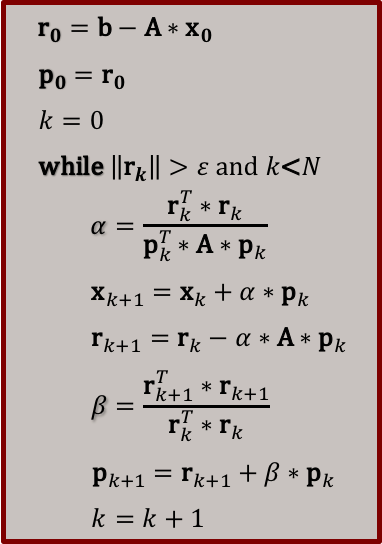
\includegraphics[scale=0.50]{figures/SPARSE-CGAlg}
      \vspace{-2em}
      \end{center}
    \column{.10\textwidth}
    \column{.45\textwidth}
      \vspace{-2em}
      \begin{center}
      \textbf{\tiny{Preconditioned Conjugate Gradient}}
      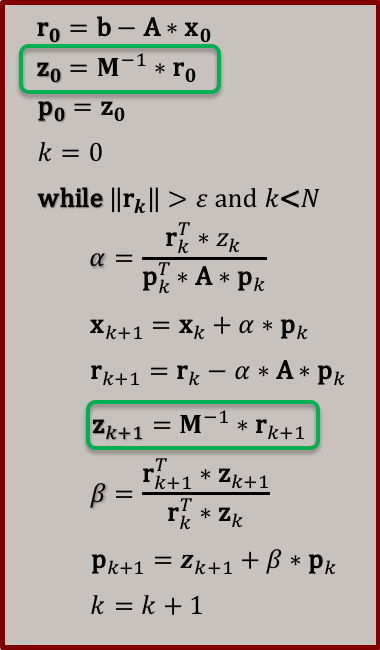
\includegraphics[scale=0.50]{figures/SPARSE-PrecondCGAlg}
      \vspace{-2em}
      \end{center}
  \end{columns}
\end{frame}

\begin{frame}[fragile]{Exercise}
\textbf{Use Case: Preconditioned Conjugate Gradient Solver}

Goal: Introduce preconditioning to a CG solver code

  \begin{columns}[t,onlytextwidth]
    \column{.55\textwidth}
      \vspace{1em}
      \\
      \begin{itemize}
      \item SPILUK: Yields factored M
      \item $M = LU \approx A$
      \item $M^{-1} = U^{-1}L^{-1}$
      \vspace{2em}
      \item SPTRSV: Apply twice for z
      \item $tmp = L \setminus r$ (Matlab notation)
    %\item Apply ILU: $\mathbf{z} = M^{-1}\mathbf{r} \Leftrightarrow z = (LU)^{-1}\mathbf{r} \Leftrightarrow z = U^{-1}(L^{-1}\mathbf{r})$
      \item $z = U \setminus tmp$
      \end{itemize}
    \column{.45\textwidth}
      \vspace{-2em}
      \begin{center}
      \textbf{\tiny{Preconditioned Conjugate Gradient}}
      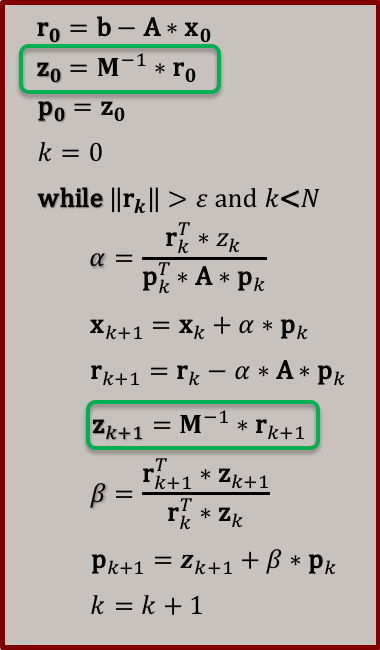
\includegraphics[scale=0.50]{figures/SPARSE-PrecondCGAlg}
      \vspace{-2em}
      \end{center}
  \end{columns}
\end{frame}

\begin{frame}[fragile]{Exercise}
\textbf{Preconditioned CG: Exercise}
\begin{itemize}
  \item Objective:
  \begin{itemize}
    \item Introduce spiluk and sptrsv as preconditioning to a CG solver
    %\item Uses a simple Laplacian matrix on a cartesian grid as a KokkosSparse::CrsMatrix
  \end{itemize}

  \item Exercise and logistics:
  \begin{itemize}
    \item \verb!Exercises/kokkoskernels/CGSolve_SpILUKprecond!
    \item For convenience, use the provided script to install KokkosKernels and generate a Makefile for the code
    \begin{code}
      run_installlibs_cmake.sh
    \end{code}
    \item Change path and build variables as needed based on your setup:
    \begin{itemize}
      \item KOKKOS\_PATH: Point to your Kokkos source directory
      \item KOKKOSKERNELS\_PATH: KokkosKernels source directory
      \item KOKKOS\_DEVICES: Enabled execution spaces
    \end{itemize}
  \end{itemize}

\end{itemize}
\end{frame}

\begin{frame}[fragile]{Exercise}
\textbf{Preconditioned CG: Exercise}
\begin{itemize}

  \item Instructions:
  \begin{itemize}
    \item Search for lines marked "EXERCISE" to apply code changes
    \item Lines marked "EXERCISE hint" give suggestions
    \item Opaque handles already created, SPILUK handle initialized
  \end{itemize}
  \item Key steps:
  \begin{itemize}
    \item Initialize two SPTRSV handles (L and U)
    \item Call spiluk\_symbolic(...) for ILU(k)
    \item Call spiluk\_numeric(...) for ILU(k) factorization
    \item Call sptrsv\_symbolic(...) to do level scheduling for L and U
    \item Call sptrsv\_solve(...) to apply preconditioner during the CGSolve
  \end{itemize}
  \item Observe the convergence behaviors:
  \begin{itemize}
    \item  without preconditioner 
    \item  with preconditioner (as ILU(k) fill-level changes)
    \item  "./cgsolve --help" will show command-line options
  \end{itemize}

\end{itemize}
\end{frame}


\begin{frame}[fragile]{Summary}
\textbf{Summary: SPILUK and SPTRSV}
\begin{itemize}
  \item SPILUK
  \begin{itemize}
    \item Two phase routine, using level scheduling to expose parallelism for the factorization
  \end{itemize}
  \item SPTRSV
  \begin{itemize}
    \item Two phase routine, using level scheduling to expose parallelism for the solve phase
    \item CuSPARSE TPL support is available for NVIDIA GPUs
  \end{itemize}
\end{itemize}

\end{frame}

%==========================================================================


%!TEX root = ../modularized/KokkosTutorial_08_KokkosKernels.tex
% \begin{frame}{DOE ECP Acknowledgement}

% \textit{
% This research was supported by the Exascale Computing Project (17-SC-20-SC),
% a joint project of the U.S. Department of Energy's Office of Science and National Nuclear Security Administration,
% responsible for delivering a capable exascale ecosystem, including software, applications, and hardware technology,
% to support the nation's exascale computing imperative.
% }

% \end{frame}

%==============================================================================

\begin{frame}[fragile]


  \vspace{10pt}
  {\Huge Building Applications with Kokkos Kernels}

  \vspace{10pt}

  \textbf{Learning objectives:}
  \begin{itemize}
    \item{Using Kokkos Kernels in Your Project}
    \item{Configure, Build, and Install Kokkos Kernels}
    \item{Install with Spack}
  \end{itemize}

%  \vspace{-20pt}
  \pause

  \begin{block}{Ignore This For Tutorial Only}
     The following details on options to integrate Kokkos into your build process are NOT necessary to know if you just want to do the tutorial.
  \end{block}

\end{frame}

\begin{frame}[fragile]{Options for Building Kokkos Kernels}

\begin{itemize}
\item \textbf{Install via CMake:} For large projects with multiple dependencies installing Kokkos via CMake and then building against it is the best option.
\item \textbf{Build inline via CMake:} This is an option suited for applications which have few dependencies (and no one depending on them) and want to build Kokkos inline with their application.
\item \textbf{Using Spack:} For projects which largely rely on components provided by the Spack package manager.
\end{itemize}
\end{frame}

\begin{frame}[fragile]{KokkosKernels CMake Basics}
\begin{itemize}
\item In the spirit of C++ for \emph{code} performance portability, modern CMake aims for \emph{build system} portability
\item Keep builds simple. Language is always C++ (even if CUDA, HIP, Sycl, ...) and all necessary flags are taken care of for you!
\item Single build system call in your project should configure everything
\vskip0.5cm
\begin{shell}
add_library(myLib goTeamVenture.cpp)
target_link_libraries(myLib PUBLIC 
                     Kokkos::kokkoskernels)
\end{shell}
\vskip0.5cm
\item No need to link to Kokkos itself. Kokkos Kernels transitively applies all Kokkos flags.
\end{itemize}
\end{frame}


\begin{frame}[fragile]{KokkosKernels CMake Basics}
\begin{itemize}
\item Developing large software tools with Kokkos requires handling transitive dependencies properly - thankfully this is fairly seamless with CMake
\item Example: abstraction layers that hide Kokkos details
\item App will still generate Kokkos code and needs all Kokkos flags
\end{itemize}
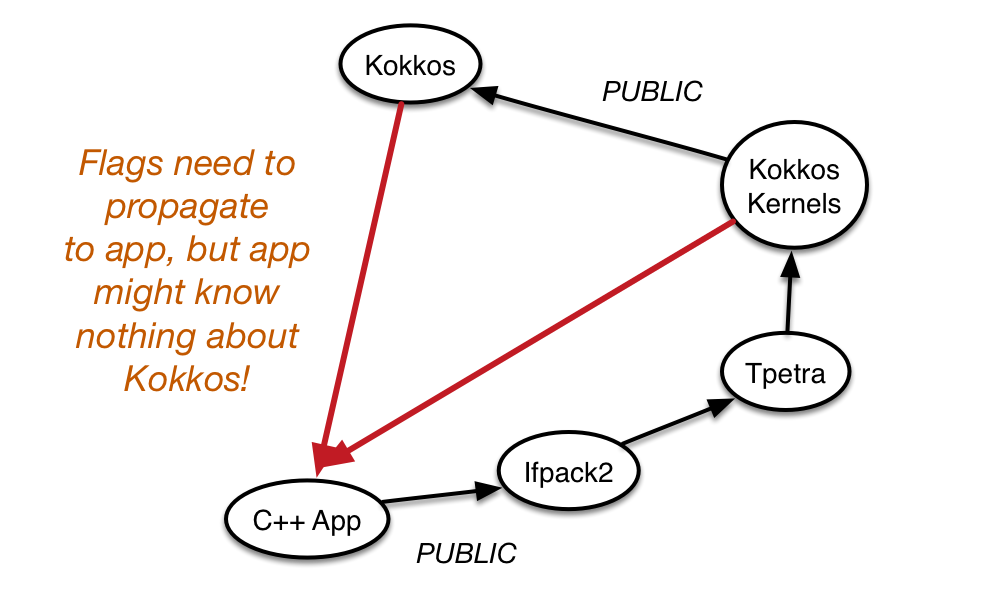
\includegraphics[width=0.6\textwidth]{../figures/DepGraphSimple.png}
\end{frame}

\begin{frame}[fragile]{Project CMake using KokkosKernels}
\textbf{Basic starting point for apps using kernels }
\begin{itemize}
\item Create a \texttt{CMakeLists.txt} file for an executable
\uncover<2-> { \item Declare your C++ project }
\uncover<3-> { \item Find Kokkos Kernels dependency }
\uncover<4-> { \item Add your program }
\uncover<5-> { \item Link to Kokkos Kernels (PRIVATE, not transitive) }
\end{itemize}

\begin{cmake}[linebackground={
  \btLstHL<2>{2}{orange!30}
  \btLstHL<3>{4}{orange!30}
  \btLstHL<4>{6}{orange!30}
  \btLstHL<5>{8-9}{orange!30}    
}]
    cmake_minimum_required(VERSION 3.12)
    project(myProject CXX) # C++ needed to build my project

    find_package(KokkosKernels REQUIRED)

    add_executable(myExe source.cpp)
    # declare dependency on KokkosKernels
    target_link_libraries(myExe PRIVATE 
                 Kokkos::kokkoskernels)
\end{cmake}
\end{frame}

\begin{frame}[fragile]{Project CMake using KokkosKernels}
\textbf{Basic starting point for app using kernels as submodule}
\begin{itemize}
\item Create \texttt{CMakeLists.txt} for a library with Kokkos built inline
\uncover<2-> { \item Declare your C++ project }
\uncover<3-> { \item Add Kokkos as a subdirectory }
\uncover<4-> { \item Add your program  }
\uncover<5-> { \item Link your program to Kokkos Kernels }
\end{itemize}

\begin{cmake}[linebackground={
  \btLstHL<2>{2}{orange!30}
  \btLstHL<3>{4-5}{orange!30}
  \btLstHL<4>{8}{orange!30}
  \btLstHL<5>{10-11}{orange!30}    
}]
    cmake_minimum_required(VERSION 3.12)
    project(myProject CXX) # C++ needed to build my project

    add_subdirectory(kokkos)
    add_subdirectory(kokkos-kernels)

    add_executable(myExe source.cpp)
    # declare dependency on KokkosKernels
    target_link_libraries(myLib PUBLIC 
                 Kokkos::kokkoskernels)
\end{cmake}
\end{frame}

\begin{frame}[fragile]{Project CMake using KokkosKernels}
\textbf{Basic starting point for helper libraries using kernels: PUBLIC dependencies}
\begin{itemize}
\item Create a \texttt{CMakeLists.txt} file for your library
\uncover<2-> { \item Declare your C++ project }
\uncover<3-> { \item Find Kokkos Kernels dependency }
\uncover<4-> { \item Add your library  }
\uncover<5-> { \item Link your library to Kokkos Kernels. Downstream apps will need Kokkos flags so linkage must be PUBLIC (i.e. transitive) }
\end{itemize}

\begin{cmake}[linebackground={
  \btLstHL<2>{2}{orange!30}
  \btLstHL<3>{4}{orange!30}
  \btLstHL<4>{7}{orange!30}
  \btLstHL<5>{9-10}{orange!30}    
}]
    cmake_minimum_required(VERSION 3.12)
    project(myProject CXX)

    find_package(KokkosKernels REQUIRED)

    add_library(myLib source.cpp)
    # declare dependency on KokkosKernels
    target_link_libraries(myLib PUBLIC 
                 Kokkos::kokkoskernels)
\end{cmake}
\end{frame}




\begin{frame}[fragile]{Configuring CMake From Command Line}
\begin{itemize}
\uncover<2-> { \item Point to your project source }
\uncover<3-> { \item Use the same C++ complier as Kokkos }
\uncover<4-> { \item Point to Kokkos Kernels installation  }
\uncover<5-> { \item Pass any Kokkos Kernels options }
\end{itemize}
\begin{shell}[linebackground={
  \btLstHL<2>{1}{orange!30}
  \btLstHL<3>{2}{orange!30}
  \btLstHL<4>{3}{orange!30}
  \btLstHL<5>{4}{orange!30}    
}]
    cmake <ProjectSourceDir> \
      -DCMAKE_CXX_COMPILER=<kokkos dir>/bin/nvcc_wrapper \
      -DKokkosKernels_ROOT=<KokkosInstallPrefix> \
      -DKokkosKernels_<OPTION>:BOOL=ON 
\end{shell}
\end{frame}

\begin{frame}[fragile]{CMake Options Overview}
\begin{itemize}
\item Options almost all fall into one of two categories
\begin{itemize}
	\item ETIs (early template instantiation) options
	\item TPLs (third-party libraries like MKL and cuBLAS)
\end{itemize}
\item Template instantiation pre-generates kernels for certain types to avoid compiler overheads later
\begin{itemize}
	\item Scalars: float, double, complex float, complex double
	\item Ordinals: int, int64\_t
	\item Offsets: int, size\_t
	\item Spaces: CUDA, OpenMP, Serial
	\item Layouts: left, right
\end{itemize}
\item Third-party libraries enable using optimized vendor implementations
\begin{itemize}
	\item MKL
	\item cuBLAS
	\item cuSPARSE
	\item SuperLU
\end{itemize}
\end{itemize}
\end{frame}

\begin{frame}[fragile]{CMake Option Examples}
\begin{itemize}
\item \inlineshell{-DKokkosKernels_INST_MEMSPACE_CUDAUVMSPACE=ON} says to pre-instantiate kernels with CUDA UVM
\item \inlineshell{-DKokkosKernels_INST_FLOAT=ON} says to pre-instantiate kernels with 32-bit floats
\item \inlineshell{-DKokkosKernels_ENABLE_TPL_MKL=ON} for MKL support
\item \inlineshell{-DKokkosKernels_ENABLE_TPL_SUPERLU=ON},  \inlineshell{-DSUPERLU_ROOT=<...>} gives install location for SuperLU
\end{itemize}

\uncover<2->{ \centering Activated options displayed in CMake output }
\begin{uncoverenv}<2->
\begin{shell}
KokkosKernels ETI Types
   Devices:  <OpenMP,HostSpace>
   Scalars:  double
   Ordinals: int
   Offsets:  int;size_t
   Layouts:  LayoutLeft

KokkosKernels TPLs
   BLAS:        /usr/lib/libblas.dylib
   LAPACK:      /usr/lib/liblapack.dylib
\end{shell}
\end{uncoverenv}
\end{frame}




\begin{frame}[fragile]{KokkosKernels via Spack: Command Line}
\begin{itemize}
\item Spack provides a package manager that automatically downloads, configures, and installs package dependencies
\item KokkosKernels itself can be easily installed with specific variants (+) and compilers (\%)
\begin{shell}
spack install kokkos-kernels@develop +openmp %gcc@8.3.0
\end{shell}
\item Good practice is to define ``best variant`` for kokkos in your packages.yaml directory, e.g. for Volta system
\begin{shell}
packages:
   kokkos:
    variants: +cuda +openmp +cuda_lambda +wrapper \
              ^cuda@10.1 cuda_arch=70
    compiler: [gcc@7.2.0]
\end{shell}
\item Build rules in \inlineshell{package.py} automatically map Spack variants to correct CMake options
\item Run \inlineshell{spack info kokkos-kernels} to see full list of variants
\end{itemize}
\end{frame}

\begin{frame}[fragile]{KokkosKernels via Spack: Package Files}
\begin{itemize}
\item Build rules created in a \inlineshell{package.py} file
\item Step 1: Declare dependency on specific version of kokkos (3.x, master, or develop)
\begin{shell}
class myLib(CMakePackage):
  depends_on('kokkos-kernels@3.2')
\end{shell}
\item Step 2: Add build rule pointing to Spack-installed Kokkos and same C++ compiler Kokkos uses
\begin{shell}
def cmake_args(self):
  options = []
  ...
  options.append('-DCMAKE_CXX_COMPILER={}'.format(
     self.spec['kokkos'].kokkos_cxx)
  options.append('-DKokkosKernels_ROOT={}'.format(
     self.spec['kokkos-kernels'].prefix)
  return options
\end{shell}
\item More details can be found in Spack.md in Kokkos repo.
\end{itemize}
\end{frame}

\begin{frame}{Section Summary}

  \begin{itemize}
    \item{Kokkos primary build system is CMake.}
    \item{Kokkos options are transitively passed on, including many necessary compiler options.}
    \item{The Spack package manager does support Kokkos.}
  \end{itemize}

\end{frame}


\begin{frame}[fragile]{Module 8: Summary}
  \textbf{Summary}
	\begin{itemize}
    \item Kokkos Kernels provides several performance portable dense, sparse, and graph kernels
    \item Working actively with vendors to incorporate algorithms in optimized vendor libraries and provide interface to them
    \item Kokkos Core, Kokkos Kernels, and Kokkos tools allows Kokkos ecosystem to be a complete solution for CSE applications
    \item Working actively with applications to address unique use cases
    \item Use slack/github/e-mail to reach out to us
	\end{itemize}
\end{frame}

\begin{frame}
{\Huge The END}

\vspace{10pt}
\begin{center}
	{\Large This concludes:}

	\vspace{20pt}
	{\Huge \textbf{The Kokkos Lectures}!}

	\vspace{20pt}
	\textit{8 Lectures -- 600 slides -- 14 hours of recording.}
\end{center}
\end{frame}

\begin{frame}[fragile]{The Kokkos Ecosystem}
  \begin{center}
    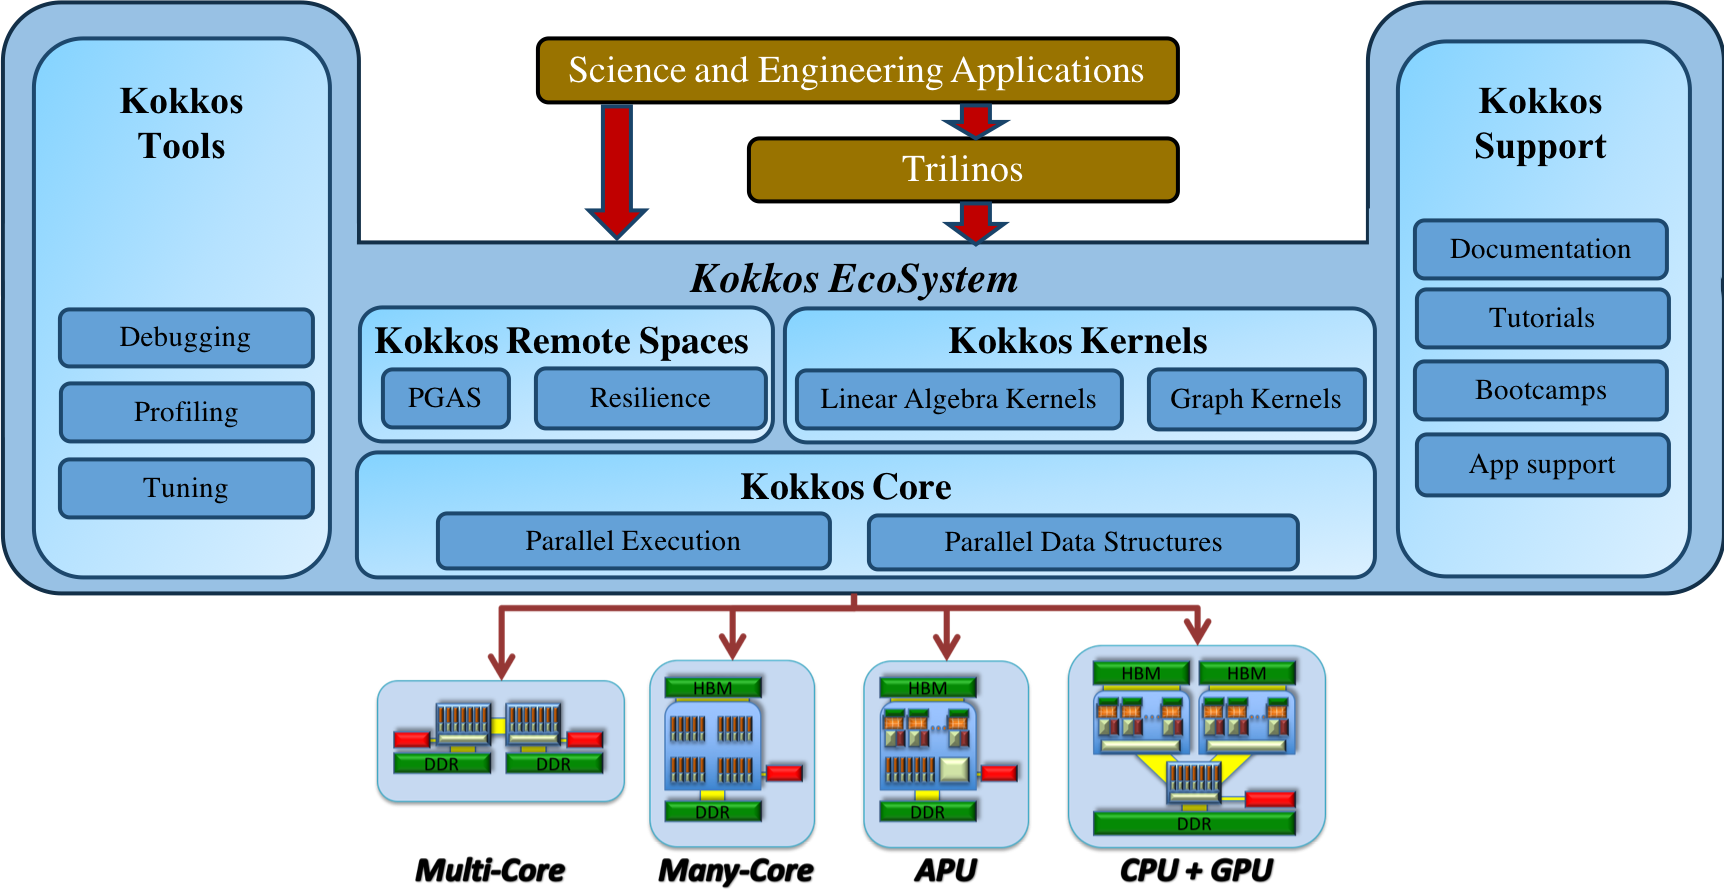
\includegraphics[width=1.05\textwidth]{figures/kokkos-eco-system}
  \end{center}
\end{frame}

\begin{frame}[fragile]{Lecture Series Outline}

\textbf{What was covered:}

\begin{itemize}
        \item Module 1: Introduction, Building and Parallel Dispatch
        \item Module 2: Views and Spaces
        \item Module 3: Data Structures + MultiDimensional Loops
        \item Module 4: Hierarchical Parallelism
        \item Module 5: Tasking, Streams and SIMD
        \item Module 6: InterOp: Python, Fortran, MPI and PGAS
        \item Module 7: Tools: Profiling, Tuning and Debugging
        \item Module 8: Kernels: Sparse and Dense Linear Algebra
\end{itemize}

\end{frame}

\begin{frame}[fragile]{The Kokkos Team}
\vspace{-5pt}
    \begin{center}
    \newcommand\placegraphics[1]{%
        \includegraphics[height=2em, width=6em, keepaspectratio]{#1}%
    }
    \placegraphics{kokkos}

    \vspace{1em}

    \begin{tabular}{cccc}
        \placegraphics{lanl} &
        \placegraphics{snl} &
        \placegraphics{anl} &
        \placegraphics{cea} \\
        \placegraphics{ornl} &
        \placegraphics{lbl} &
        \placegraphics{cscs} &
        \\
    \end{tabular}
\end{center}

\vspace{-5pt}
	\begin{scriptsize}
	\begin{tabular}{p{0.20\textwidth} p{0.8\textwidth} }
		\textbf{Kokkos Core:} & \textbf{C.R.Trott}, J. Ciesko, V. Dang, N. Ellingwood, D.S. Hollman, D. Ibanez, J. Miles, J. Wilke, 
		, H. Finkel, N. Liber, D. Lebrun-Grandie, D. Arndt, B. Turcksin, J. Madsen, R. Gayatri \\
		& \texttt{former:} H.C. Edwards, D. Labreche, G. Mackey, S. Bova, D. Sunderland \\
		\textbf{Kokkos Kernels:} & \textbf{S. Rajamanickam}, L. Berger, V. Dang, N. Ellingwood, E. Harvey, B. Kelley, K. Kim, C.R. Trott, J. Wilke, S. Acer \\
		& \texttt{former:} M. Deveci, M. Hoemmen, A. Bradley \\
		\textbf{Kokkos Tools} & \textbf{D. Poliakoff}, C. Lewis, S. Hammond, D. Ibanez, J. Madsen, S. Moore, C.R. Trott \\
		\textbf{Kokkos Support} & \textbf{C.R. Trott}, G. Shipmann, G. Womeldorff, and all of the above \\
		& \texttt{former:} H.C. Edwards, G. Lopez, F. Foertter, J. Amelang
	\end{tabular}
	\end{scriptsize}
\end{frame}

\begin{frame}[fragile]{Acknowledgements}

\textbf{H. Carter Edwards}: who started this all!

\vspace{10pt}
\textbf{Mike Heroux}: for believing in Kokkos and being a champion for the project in its early phase.

\vspace{10pt}
\textbf{Jeff Amelang}: who developed the original tutorial material 2015.

\vspace{10pt}
\textbf{Sandia LDRD program}: which did the initial funding of Kokkos.

\vspace{10pt}
\textbf{DOE Exascale Computing Project}: for funding training efforts and the expansion of the Kokkos team to more institutions.
\end{frame}

\begin{frame}[fragile]{Welcome to Kokkos}

\textbf{Online Resources}:

\begin{itemize}
        \item \url{https://github.com/kokkos}:
                \begin{itemize}
                        \item Primary Kokkos GitHub Organization
                \end{itemize}
        \item \url{https://github.com/kokkos/kokkos-tutorials/wiki/Kokkos-Lecture-Series}:
                \begin{itemize}
			\item{Slides, recording and Q\&A for the Lectures}
                \end{itemize}
        \item \url{https://github.com/kokkos/kokkos/wiki}:
                \begin{itemize}
                        \item Wiki including API reference
                \end{itemize}
        \item \url{https://kokkosteam.slack.com}:
                \begin{itemize}
                        \item Slack channel for Kokkos.
                        \item Please join: fastest way to get your questions answered.
                        \item Can whitelist domains, or invite individual people.
                \end{itemize}
\end{itemize}

\end{frame}


\end{document}

